\documentclass[12pt]{article}

\usepackage[ngerman]{babel}
\usepackage[utf8x]{inputenc}
\usepackage{amsmath}
\usepackage{graphicx}
\usepackage[colorinlistoftodos]{todonotes}
\usepackage{listings}
\usepackage{glossaries}
\usepackage{placeins}
\usepackage{fixltx2e}
\usepackage{pdfpages}
\usepackage{lastpage}
\usepackage{enumitem}
\usepackage{xcolor}
\usepackage{scrpage2}
\usepackage{scrtime}
\usepackage{parskip}
\usepackage{hyperref}
\usepackage{titlesec}

\clearscrheadfoot
\pagestyle{scrheadings}
\usepackage[
top    = 2.5cm,
bottom = 3cm,
left   = 3cm,
right  = 3cm]{geometry}
\setcounter{secnumdepth}{4}
\title{Diplomarbeit}


\author{DigitalSchoolNotes}
\date{\today}

%Paragraph Format
\titleformat{\paragraph}
{\normalfont\normalsize\bfseries}{\theparagraph}{1em}{}
\titlespacing*{\paragraph}
{0pt}{3.25ex plus 1ex minus .2ex}{1.5ex plus .2ex}

%Includes
\setlength{\parindent}{0cm}

\newcommand{\executeiffilenewer}[3]{%
\ifnum\pdfstrcmp{\pdffilemoddate{#1}}%
{\pdffilemoddate{#2}}>0%
{\immediate\write18{#3}}\fi%
}
\newcommand{\includesvg}[1]{%
\executeiffilenewer{#1.svg}{#1.pdf}%
{inkscape -z -D --file=#1.svg --export-pdf=#1.pdf --export-latex}%
\input{#1.pdf_tex}[width=1.0\textwidth]%
}

%Bibtex
\def\BibTeX{{\rm B\kern-.05em{\sc i\kern-.025em b}\kern-.08em
		T\kern-.1667em\lower.7ex\hbox{E}\kern-.125emX}}

%lslisting
\lstdefinelanguage{Javascript}{
  keywords={typeof, new, true, false, catch, function, return, null, catch, switch, var, if, in, while, do, else, case, break},
  keywordstyle=\color{blue}\bfseries,
  ndkeywords={class, export, boolean, throw, implements, import, this},
  ndkeywordstyle=\color{darkgray}\bfseries,
  identifierstyle=\color{black},
  sensitive=false,
  comment=[l]{//},
  morecomment=[s]{/*}{*/},
  commentstyle=\color{purple}\ttfamily,
  stringstyle=\color{red}\ttfamily,
  morestring=[b]',
  morestring=[b]"
}

\lstdefinestyle{customjava}{
  	language=Java,
  	frame=tlrb,
  	aboveskip=3mm,
  	belowskip=6mm,
  	showstringspaces=false,
  	columns=flexible,
  	basicstyle={\small\ttfamily},
  	numbers=none,
  	numberstyle=\tiny\color{gray},
  	keywordstyle=\color{purple},
  	commentstyle=\color{orange},
  	stringstyle=\color{blue},
  	breaklines=true,
  	breakatwhitespace=true
  	tabsize=3,
  	captionpos=b,
}



\lstset{escapechar=@,style=customjava}

%Cite right
\newcommand{\citeof}[2]{{
		\par \begingroup \leftskip=1cm \noindent \textit 
		''#1'' \cite{#2} \\
		\par \endgroup
	}}
	
% Picture insert (UseCase)
% \insertpicture{mik.png}{Some picture}{\cite{bk_key}}{itm:pic1}{0.5}
\newcommand{\insertpicture}[5]{{
	\begin{figure}[!htb]
		\centering\includegraphics[width=#5\textwidth]{#1}
		\ifthenelse{\equal{\unexpanded{#3}}{(selfmade)}}{\caption[#2]{#2}}{\caption[#2 #3]{#2 #3}}
		
		\label{#4}
	\end{figure}
	\FloatBarrier
}}
\makeglossaries
\newglossaryentry{json} {name=JSON, description={Java Script Object Notation}}
\newglossaryentry{Stakeholder} {name=Stakeholder, description={Eine Person welche Interesse am Ergebnis des Projektes hat, jedoch nicht an der Entwicklung des Projektes an sich beteiligt ist.}}
\newglossaryentry{Latenz} {name=Latenz, description={Verzögerung zwischen Anfrage und Antwort(Ping)}}
\newglossaryentry{TGM} {name=TGM, description={Technologisches Gewerbe Museum}}
\newglossaryentry{IDE} {name=IDE, description={Integrated Development Environment}}
\newglossaryentry{KVM} {name=KVM, description={Kernel-based Virtual Machine}}
\newglossaryentry{SSH} {name=SSH, description={Secure Shell}}
\newglossaryentry{DNS} {name=DNS, description={Domain Name Service}}
\newglossaryentry{HTTP} {name=HTTP, description={Hypertext Transfer Protocol}}
\newglossaryentry{HTTPS} {name=HTTPS, description={Hypertext Transfer Protocol Secure}}
\newglossaryentry{SSL} {name=SSL, description={Secure Sockets Layert}}
\newglossaryentry{API} {name=API, description={Application Programming Interface}}
\newglossaryentry{WSGI} {name=WSGI, description={Web Server Gateway Interface}}
\newglossaryentry{DSN} {name=DSN, description={Digital School Notes}}

\renewcommand*\glspostdescription{\dotfill}




\begin{document}


\begin{titlepage}
\begin{center}

% Deckblatt

\includegraphics[width=0.25\textwidth]{images/dsn_logo}\\
\vspace{5mm}

\LARGE TGM - HTBLuVA Wien XX \\ IT Abteilung  \\[1.5cm]

% Titel
\rule{1.0\textwidth}{1mm}
{ \huge \bfseries \\[0.4cm]  \huge Diplomarbeit \\ \LARGE DigitalSchoolNotes \\[0.4cm] }

\rule{1.0\textwidth}{1mm}



\noindent 


\vfill

% Fusszeile
{\small Version: \today ~um  \thistime    }
\end{center}

%\end{center}
\end{titlepage}


%HEADER AND FOOTER
\pagenumbering{Roman}
\ohead{\headmark}
\ifoot{© DigitalSchoolNotes - 2015/16}
\ofoot{\pagemark}

\newpage %----------------------------------------------------------------------------------------------
{\small\color{white}.}
\vspace{-0.7cm}
\renewcommand*\contentsname{Inhalt}
\tableofcontents

\newpage %----------------------------------------------------------------------------------------------
% Erklärung
%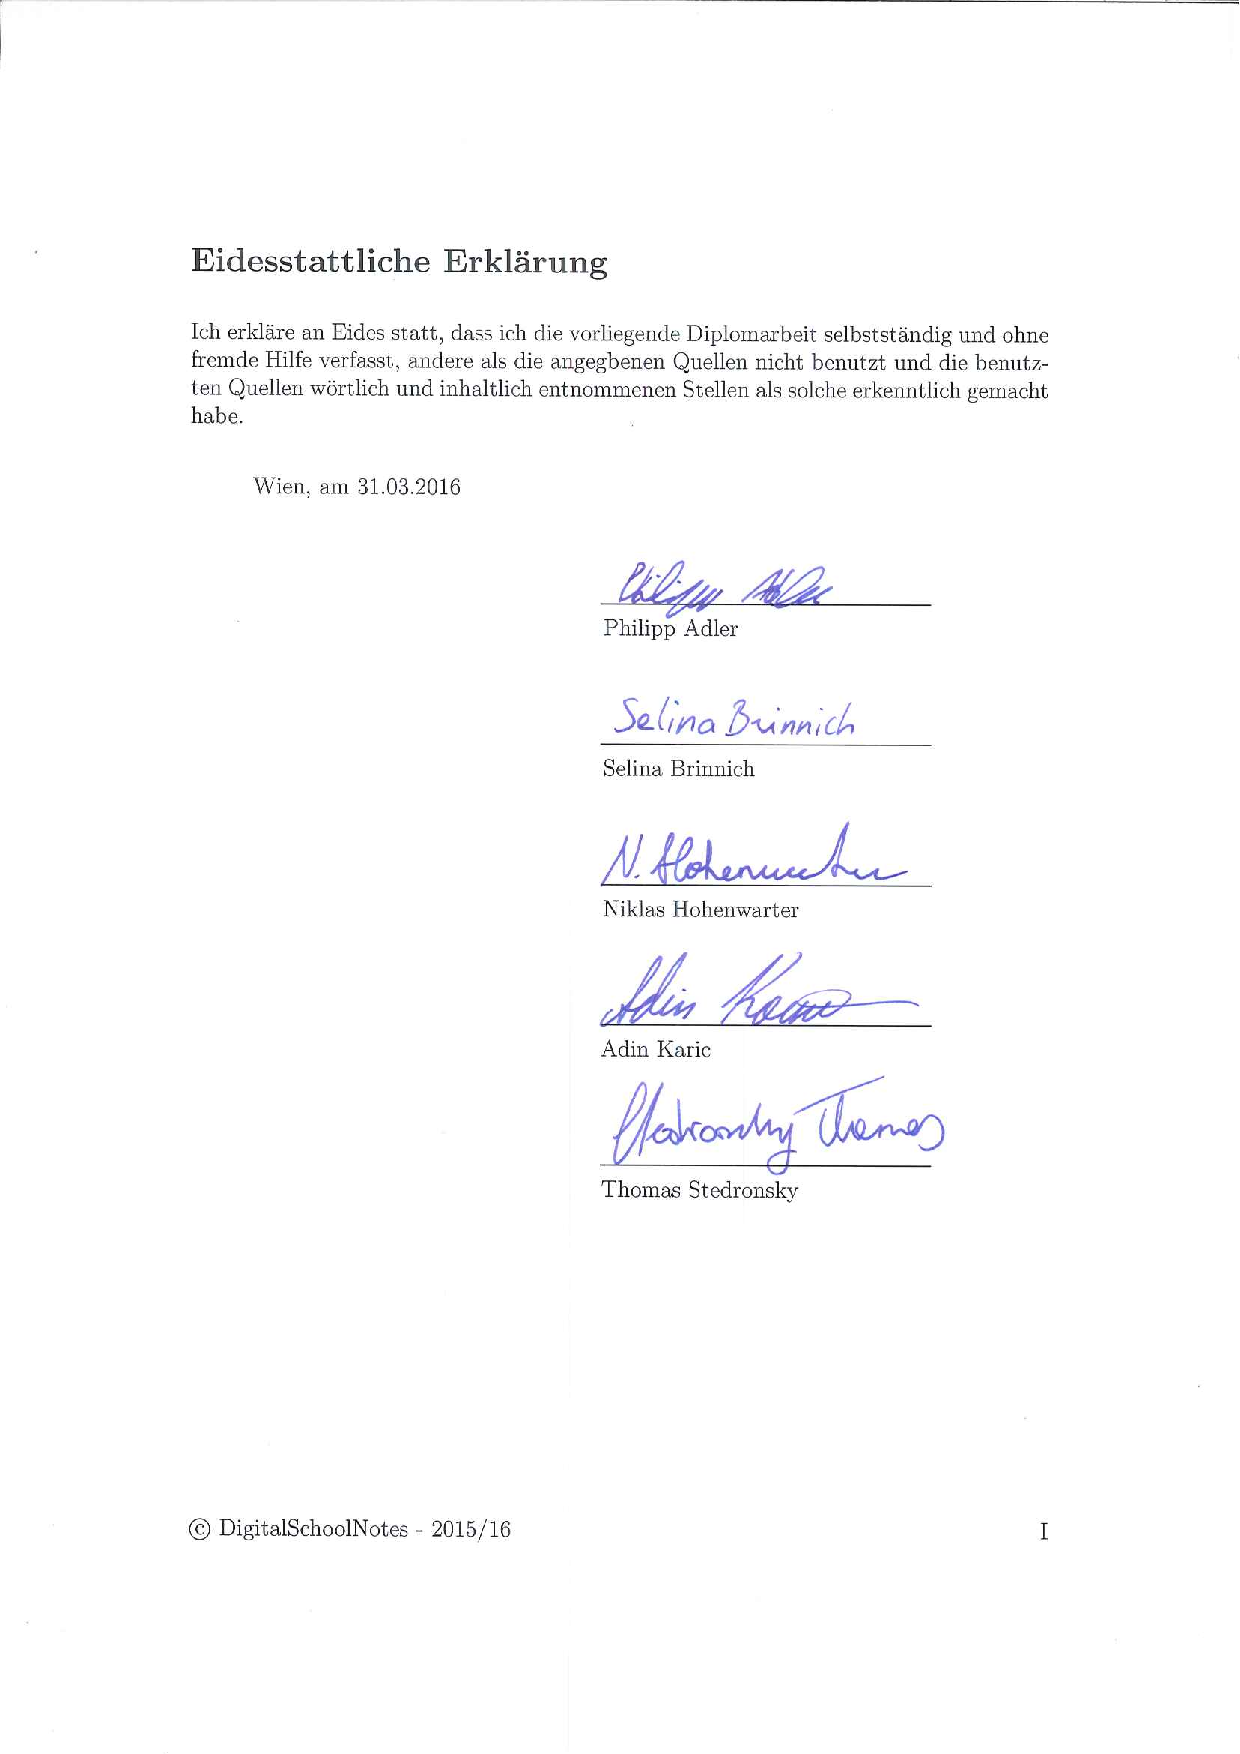
\includepdf[scale=1.2,pages=-]{documents/erklaerung}


\section*{Eidesstattliche Erklärung}
Ich erkläre an Eides statt, dass ich die vorliegende Diplomarbeit selbstständig und ohne fremde Hilfe verfasst, andere als die angegbenen Quellen nicht benutzt und die benutzten Quellen wörtlich und inhaltlich entnommenen Stellen als solche erkenntlich gemacht habe. \\

Wien, am 30.03.2016 \\ \\ \\

Philipp Adler \\ \\ \\

Selina Brinnich \\ \\ \\

Niklas Hohenwarter \\ \\ \\

Adin Karic \\ \\ \\

Thomas Stedronsky

\newpage
\section*{Abstract}
\cfoot{Selina Brinnich}

Nowadays most people can't think of a world without internet anymore. It is used almost always and everywhere you are - also in schools. Students are getting more and more into digital notes, especially in technical oriented schools, where they have their laptop always with them. There is only one problem: These digital notes are often written in different programs. They are unorganized and mostly left in some directory where they aren't opened once afterwards.\\
The project DigitalSchoolNotes was formed exactly because of this problem. Our web-application can organize digital notes and make it easier to write them. It is made from students themselves to fit the needs of students optimal. The application can be accessed from almost every device - personal computers, laptops and even tablets. Furthermore it is possible to use a mobile phone to take a photo and put it into the digital notes easy and conveniently. Particularly fitted for technical schools there is also the possibility to insert some code-snippets into the digital notes, which are correctly formatted and highlighted.\\
All of which is to allow students to write tidy, organized, digital notes and to make learning from these easier and more efficient.
\section*{Kurzfassung}
\cfoot{Selina Brinnich}

Die heutige digitale Welt ist aus den Köpfen der meisten Menschen gar nicht mehr wegzudenken. Das Internet wird beinahe immer und überall verwendet - so auch immer mehr in Schulen. Vor allem in technischen Schulen werden Mitschriften aus dem Unterricht immer öfters digitalisiert. Das Problem dabei: Diese Mitschriften werden meist in unterschiedlichen Programmen verfasst, sie sind unorganisiert und verenden oft in irgendeinem Ordner ohne jemals wieder angesehen zu werden.\\
Das Projekt DigitalSchoolNotes setzt genau bei diesem Problem an. Unsere Web-Applikation soll das Führen einer digitalen Mitschrift einfacher und organisierter machen. Dabei wollen wir speziell auf die Bedürfnisse der Schüler eingehen. Der Zugriff auf die Applikation ist sowohl von Desktop Systemen und Laptops, als auch von Tablets über eine Webseite möglich. Ein eingeschränkter Zugriff ist zudem für Handys möglich, um beispielsweise Tafelbilder schnell und bequem in die Mitschrift einfügen zu können. Speziell für technisch orientierte Schulen gibt es auch die Möglichkeit, Teile von Programmcode richtig formatiert erstellen zu können. \\
Das alles dient dazu, Schülern eine ordentliche, organisierte, digitale Mitschrift zu erleichtern und das Lernen aus diesen einfacher und effizienter zu gestalten.
\newpage
\section*{Danksagungen}
\cfoot{}

%Text...
\label{pageRomanEnd}


\newpage %----------------------------------------------------------------------------------------------

\pagenumbering{arabic}
\ofoot{\pagemark}

\section{Einleitung}
\label{sec:einleitung}
%\section*{Einleitung}
\cfoot{Niklas Hohenwarter}

Am Anfang des Diplomprojektes Digital School Notes (\gls{DSN}) stand der Ideenfindungsprozess. Das Team wollte an einem sinnvollen Diplomprojekt arbeiten, also ein Projekt, welches nachher weitergeführt werden und verkauft werden könnte. Durch diese Art von Projekt versprach sich das Team eine höhere Arbeitsmoral. 

Die Idee kam während einer Unterrichtsstunde. Mal wieder schrieb niemand mit und kaum einer passte auf. Man hatte schon länger versucht eine Idee für ein Diplomprojekt zu finden und auf einmal war es doch so offensichtlich. Das Diplomprojekt sollte den Alltag in der Schule verbessern. Da kam die Idee für Digital School Notes.

Was, wenn mitschreiben auf einmal wieder interessanter ist? Wenn die Mitschrift am Laptop geführt wird und nicht mehr am Papier? Das würde so vieles einfacher machen. Ein digitales Schulheft. Sofort begannen wir die technische Machbarkeit zu prüfen. Die Software müsste eine Web Applikation sein um alle Betriebssysteme zu unterstützen. Sie müsste leicht zu bedienen und komfortabel sein. Es müsste möglich sein mehrere Schulen zu unterstützen, um eine große Userbase aufzubauen. Und natürlich müsste die Software attraktiv genug sein, um zahlende Kunden anzulocken und somit die Kosten der Infrastruktur decken zu können.

Nachdem die Idee fest stand wurde ein Lastenheft verfasst. Mit diesem Lastenheft hat das Team dann mehrere Lehrer kontaktiert, um weitere Ideen und Verbesserungsvorschläge einzuholen. Die Resonanz war gut, was das Team umso mehr motivierte. Das Projekt wurde genehmigt und die Implementierung begann.

Diese Diplomarbeit fasst die Arbeit am Projekt zusammen. Sie gibt Aufschluss über die Probleme und Lösungen, an welchen das Team gearbeitet hat.

\newpage

\section{Problembeschreibung}
\label{sec:problembeschreibung}
%\section*{Problembeschreibung}
\cfoot{Niklas Hohenwarter}

Im Schulunterricht mitzuschreiben ist wichtig, jedoch immer weniger Schüler machen dies auch. Falls sie doch mitschreiben, dann verschwindet der Zettel oder Collegeblock meistens oder ist im entscheidenden Moment nicht zur Hand. Es ist kompliziert den, in immer größeren Teilen, digital ablaufenden Unterricht auf Papier festzuhalten und seine Mitschriften zu organisieren. Als Resultat dieser Umstände wird die händisch geführte Mitschrift langsam aber sicher aussterben. \\

Statt der händischen Mitschrift wird die digitale Mitschrift am im Unterricht verwendeten Laptop immer beliebter. Diese hat allerdings bis heute ähnliche Probleme. Es ist kompliziert die Struktur des Tafelbildes in z.B. ein Word-File zu übernehmen. Außerdem passiert es häufig, dass die Datei welche die Mitschrift enthält nicht mehr gefunden wird oder einfach einen unpassenden Dateinamen hat, welcher nicht die entsprechende Mitschrift vermuten lässt. Mit am Markt erhältlichen Produkten ist es ebenfalls mühsam digital mitzuschreiben.

\subsection{Umfeldanalyse}
\label{subsec:umfeldanalyse}
%\section*{Umfeldanalyse}
\cfoot{Niklas Hohenwarter}

Es existiert bereits einiges an Software welche sich mehr oder weniger dafür eignet digital mitzuschreiben. Die Features der einzelnen Produkte sind großteils bekannt, deshalb werden diese nur oberflächlich beschrieben:

\begin{itemize}
\item \textbf{Microsoft Word:} Am weitesten verbreitete Textverarbeitungssoftware; kostenpflichtig; auf Windows, Mac, Android \& iOS verfügbar
\item \textbf{Libre Office Writer:} Textverarbeitung; OpenSource; kostenlos; auf Windows, Mac \& Linux verfügbar
\item \textbf{OpenOffice Writer:} Textverarbeitung; OpenSource; kostenlos; auf Windows, Mac \& Linux verfügbar
\item \textbf{Kingsoft WPS Writer:} Textverarbeitung; kostenlos oder kostenpflichtig; auf Windows, Mac, Android \& iOS verfügbar; sehr stark an Microsoft Word angelehnt
\item \textbf{Microsoft OneNote:} Notizprogramm; Notizen können beliebig platziert und angeordnet werden; Organisation in Notizbüchern; gleichzeitiges Bearbeiten möglich; auf Windows, Mac, Android \& iOS verfügbar; kostenlos
\item \textbf{Google Docs:} Textverarbeitung; kostenlos; Betriebssystemunabhängig (Browser); gleichzeitiges Arbeiten mögliich
\end{itemize}

\newpage

\subsection{Projektidee}
\label{subsec:projektidee}
%\section*{Projektidee}
\cfoot{Adin Karic}
Die Idee hinter dem Diplomprojekt ,,Digital School Notes" war es eine Web-Applikation zur Führung einer digitalen Mitschrift zu entwickeln. Der Zugriff und das Bearbeiten soll von Desktop Systemen, Laptops und Tablets über eine Website möglich sein. Des Weiteren soll die Applikation mit Ausnahme der Heftbearbeitung auch auf Handys verfügbar sein. Das System sollte eine hohe Verfügbarkeit und gleichzeitig, für Schüler optimiert, eine leichte Bedienung bieten. 

Es sollte ein System entwickelt werden, welches extra auf die Bedürfnisse von Schülern angepasst ist. Das Produkt soll es ermöglichen, ganz einfach und schnell verschiedene externe Medien, wie zum Beispiel Bilder, Links auf andere Webseiten oder Code-Snippets in ein ,,Heft'' einzufügen und zu verwalten. Durch eine sehr simpel gestaltete Benutzeroberfläche sollte die Bedienung zum Einfügen solcher Medien, im Vergleich zu anderen Produkten auf dem Markt, deutlich vereinfacht werden. Das Anbieten von verschiedenen Dateiformaten, sowie der sichere Umgang mit den Daten der Nutzer war ebenso ein Anliegen.

Durch einen eigenen Stundenplan sollte das Rundumpaket, welches wir den Schülern bieten wollen, zusätzlich bereichert werden. Der Nutzer kann im Stundenplan die Dauer, sowie die Anfangs- und Endzeit der jeweiligen Unterrichtseinheiten festlegen. Des Weiteren kann er dann die entsprechenden Einheiten im Stundenplan eintragen. Diese Angaben sind beliebig oft änderbar. Beim Klick auf eine der eingetragenen Unterrichtseinheiten soll sich dann automatisch das dazugehörige Heft des Users öffnen (wenn zuvor ein Heft dieser Unterrichtseinheit bzw. diesem Fach zugeteilt wurde).

Schüler sollten einfach Bilder hochladen und den Text aus den Bildern automatisch in ihr Heft einfügen können. Dies sollte mit Optical Character Recognition (optische Zeichenerkennung) ermöglicht werden. Das OCR-System sollte ein Bild des Users entgegennehmen, dieses mit OCR-Algorithmen analysieren und schließlich den aus dem Bild erkannten Text in das Heft einfügen. Somit soll den Schülern ein vereinfachtes Einfügen von gedruckten Angaben oder Hausübungen, welche dann direkt bearbeitbar sind, ermöglicht werden.

Da Gruppenarbeiten und Referate im schulischen Bereich keine Seltenheit sind, wurde auch an eine Optimierung in dieser Hinsicht gedacht. Durch ein eigenes ,,Parallel Working System'' sollte das gemeinsame Arbeiten für Schüler deutlich vereinfacht werden. Jeder Schüler soll die Möglichkeit haben, einige seiner Hefte mit anderen Schülern zu teilen. Diese geteilten Hefte können dann von allen dazu berechtigten Nutzern bearbeitet werden. Ein besonderes Augenmerk ist dabei auf die Konsistenz der bearbeiteten Hefte zu legen. Durch verschiedene Sperrmechanismen muss die Integrität der Daten in den geteilten Heften gesichert werden.

\newpage

Um mit dem Produkt Geld zu verdienen, sind nach einer kostenlosen Probezeit von 90 Tagen kostenpflichtige Benutzerkonten vorgesehen. Die Nutzer sollen also nach der Probezeit einen geringen monatlichen Betrag entrichten, um das Produkt nutzen zu können. Zusätzlich ist der Vertrieb des Produkts an Schulen angedacht. Diese würden dann einen gewissen Betrag pro erworbener Lizenz zahlen, wobei diese Lizenz dann nicht zeitlich begrenzt ist und das Hosting auf den Servern der jeweiligen Schule stattfindet. Als zusätzliche Einnahmequelle könnte man noch, in Kooperation mit verschiedenen Werbenetzwerken, Werbung auf der Webseite schalten. Dabei wäre, aufgrund der vergleichsweise langen Verweildauer, die Seite der Heftansicht ein interessanter Platz für eine klassische Bannerwerbung oder Ähnliches.


\subsection{Projektkoordination}
\label{subsec:projektkoordination}
%\section*{Projektkoordination}
\cfoot{Adin Karic}

%Text...
\subsubsection{Kurzeinführung in Scrum}

\subsubsection{Scrum im Team}

\newpage
%----------------------------------------------------------------------------------------------

\section{Stand der Technik}
\label{sec:standdertechnik}

\subsection{Frameworks}
\label{subsec:frameworks}
%\section*{Frameworks}
\cfoot{Philipp Adler}

Frameworks stellen die Grundstruktur für die Entwicklung von Programmen zur Verfügung. Sozusagen ermöglichen sie durch vordefinierte Grundbausteine eine schnelle, reibungslose Entwicklung. Mithilfe von Schnittstellen und Bibliotheken soll dem Entwickler Arbeit abgenommen werden. Anforderungen, wie Kommunikation mit anderen Systemen, Imports und Validierung von Daten, werden dank des Frameworks automatisch im Hintergrund abgewickelt.

Die nachfolgenden Frameworks wurden auf einer Linux-Distribution installiert, sowie konfiguriert und getestet.\\
Für unser System benötigen wir:
\begin{itemize}
\item ein \textbf{Web Framework} als Grundgerüst
\item ein \textbf{JS-Framework} um auf Useraktionen zu reagieren
\item ein \textbf{\gls{CSS}-Framework} für das grafische Design
\item \textbf{Element-Frameworks} als Grundlage für die Funktionen in den Schulheften
\item \textbf{GUI-Testing} um zu garantieren, dass die Funktionen reibungslos laufen
\end{itemize}

\newpage

\subsubsection{Web Frameworks}
Web Frameworks haben das Ziel, dem Entwickler einer Webanwendung mit Hilfe von vordefinierten Klassen zu unterstützen. Sie sorgen dafür, dass eine Verbindung mit der Datenbank aufgebaut wird, Inhalte dynamisch angezeigt werden und ein Anmeldesystem zur Verfügung steht.\\
Web Frameworks teilen das Projekt in zwei Teile, dem Backend und Frontend.\\
Für die Auswahl unserer Web Frameworks wurden Flask, Django und Play verglichen. Da sich das Team für die Backend-Programmiersprache Python entschieden hat, stand von vornherein ein eingeschränktes Angebot an Web Frameworks zur Verfügung. Von jeder Kategorie, Full-Stack-Framework, Non-Full-Stack-Framework und micro-Framework, wurde das meist verwendeste ausgewählt. 

Dabei wurde beachtet, wie aufwendig die Installation und Konfiguration ist, wie weit es ausbaufähig ist und welche Funktionalität bereits zur Verfügung steht.

\paragraph{Flask}
\textit{,,Flask ist ein microframework für Python, basierend auf Werkzeug, Jinja 2.''}\cite{FLASK} Es ist frei verfügbar und aufgrund seiner geringen Größe schnell und einfach zu installieren und konfigurieren. Da es zu den kleineren Web Frameworks zählt, wird wenig Funktionalität geboten, welche aber durch einfache Erweiterungen behoben werden kann.\cite{FLASK}

Die Installation von Flask ist ziemlich simpel. Es kann mit folgendem Befehl installiert werden:
\begin{lstlisting}[caption={Installation von Flask \cite{FLASK}}, language=bash]
pip3 install Flask
\end{lstlisting}

\newpage

Für ein einfaches ,,Hello World''-Programm, geschrieben in Flask, braucht es eine Funktion, die die Nachricht ,,Hello World'' ausgibt und eine Main-Methode, welche die Applikation startet.

\begin{lstlisting}[caption={Flask Hello-World \cite{FLASK}}, escapeinside={(*}{*)}, language=Python]
from flask import Flask

app = Flask(__name__)#__name__ ist der Name der Applikation

@app.route("/")#definiert die URL, welche die Funktion aufruft
def hello():
	return "Hello Flask World!"

if __name__ == "__main__":
    app.run()
\end{lstlisting}

Mit dem Befehl \textit{python3 hello.py} lässt sich das Programm ausführen. Bei Aufruf der oben angeführten Adresse erscheint ,,Hello Flask World'' auf dem Bildschirm.

\paragraph{Django}
Django ist ein Open-Source Python Web Framework für die Entwicklung einer Webanwendung. Es bietet eine detaillierte und umfangreiche Dokumentation über alle Funktionalitäten und wird außerdem durch eine große Community unterstützt. Obwohl es mit sehr vielen Features ausgestattet ist, ist es einfach erweiterbar und kann mit wenig Aufwand installiert und konfiguriert werden. Außerdem unterstützt Django eine Reihe von Document Object Model-Dateitypen, wie xml, json und yaml. \cite{DJANGO}

Installiert wurde das Web Framework folgenderweise:
\begin{lstlisting}[caption={Installation von Django\cite{DJANGOIN}}, language=bash]
apt-get install python3-django
\end{lstlisting}

\newpage

Zur Erstellung eines ,,Hello-World''-Programmes muss zu Beginn ein Projekt erzeugt werden. Im nächsten Schritt ist die Datenbank entsprechend der Project-Settings zu konfigurieren. Anschließend wird im Unterordner \textit{app} ein neues File ,,hello.py'' mit folgenden Code erstellt:

\begin{lstlisting}[caption={Django Hello-World \cite{DJANGOCODE}}, language=Python]
from django.http import HttpResponse

def hello_world(request):
	return HttpResponse("Hello Django World!")
\end{lstlisting}

Wird der Server mit dem Befehl \textit{python manage.py runserver} gestartet, erscheint ,,Hello World'' im Browserfenster.

\paragraph{Play}
Play, ein leichtgewichtiges Web Framework basierend auf Java und Scala, steht für den kommerziellen Gebrauch kostenlos zur Verfügung. Allerdings ist die herstellerspezifische Dokumentation nicht besonders ausführlich.\\
Die Installation gestaltete sich im Vergleich zu anderen Web Frameworks zeitaufwendiger. \cite{PLAY}

Um Play zu installieren muss das Framework zunächst von
\textit{https://www.playframework.com/download} heruntergeladen werden. Das downgeloadete zip-File muss entpackt und der darin enthaltene Activator zum PATH hinzugefügt werden. Danach wird der Activator mit folgendem Befehl gestartet\cite{PLAYCON}:
\begin{lstlisting}[caption={Konfiguration von Play \cite{PLAYCON}}, language=bash]
activator ui
\end{lstlisting}

Für das ,,Hello-World''-Programm braucht es ein neues Projekt. Im Unterordner \textit{/controllers} muss folgende Methode hinzugefügt werden:

\begin{lstlisting}[caption={Play Hello-World \cite{PLAYCON}}]
public static Result hello() {
	return ok(main.render("Hello World",new
		play.twirl.api.Html("Hello Play World!")));
}
\end{lstlisting}

Zu guter Letzt wird der Prototyp mit dem Befehl \textit{activator run} im Projekt-Verzeichnis ausgeführt.

\paragraph{Vergleich}
Das Team hatte im Vorfeld mit der Programmierung von Web Frameworks noch keine Erfahrungswerte. \\
Aufgrund der leicht verständlichen Dokumentation, der zahlreichen Funktionialitäten wie Authentifikation, REST API, sowie der gut vernetzten Community und hat sich Django klar herauskristallisiert. Als wichtige Entscheidungshilfe galten die erstellten Prototypen. Die schnelle, einfache Entwicklung, sowie die Installation und Konfiguration des Frameworks, hinterließ beim Team einen guten Eindruck.

\subsubsection{JS-Frameworks}
JavaScript-Frameworks werden verwendet, um Benutzereingaben entgegenzunehmen, diese Daten zu validieren und zu verarbeiten und am Ende das Ergebnis zu retounieren.\\
Im Falle von DSN dienen sie als Schnittstelle zum Webserver und außerdem dazu, den Inhalt dynamisch zu ändern. Verglichen wurden die bekanntesten, populärsten JavaScript-Frameworks in den Bereichen:
\begin{itemize}
\item Browserunterstützung
\item Dokumentation \& Community
\item Lizenz und Kosten
\item Schwierigkeit bei der Erstellung eines Prototypen
\end{itemize}
\paragraph{Dojo}
Dojo ist eine frei anwendbare JS-Bibliothek von Dojo Foundation, die Entwicklern JS- und Ajax-basierende Module anbietet. Das Framework ist modular aufgebaut, sodass für eine gute Übersicht im Code gesorgt ist. Die Dokumentation besteht aus einer übersichtlichen Auflistung von step-by-step Tutorials. \cite{DOJO}

Für das Installieren bzw. Anwenden des Frameworks gibt es zwei Möglichkeiten. Die eine besteht darin, den gesamten Source-Ordner herunterzuladen, in dem sich die Kernfunktionalitäten befinden. Oder ganz einfach den Link der \textit{dojo.js} Datei im Header anzugeben.
\begin{lstlisting}[caption={Dojo einbinden\cite{DOJODOWN}}, language=HTML]
<script src="//ajax.googleapis.com/ajax/libs/dojo/1.10.4/dojo/dojo.js">
</script>
\end{lstlisting}

Der Prototyp, ein Drag \& Drop Beispiel, ließ sich dank verständlicher Erklärung ohne Probleme umsetzen. Allerdings muss sich der Entwickler im Klaren sein, welche Module für eine lauffähige Applikation einzubinden sind. \cite{DOJO}

\paragraph{Sencha ExtJS}
Das ExtJS JavaScript Framework von Sencha dient der Realisierung von komplexeren Anwendungen. Sencha bietet eine gut ausgebaute, strukturierte API. Neben einer großen Community von über 500.000 Mitgliedern unterstützt ExtJS alle marktführenden Webbrowser, sowie Smartphones.\\
Sencha ist unter der Commercial License oder GNU General Public License verfügbar. Für den kommerziellen Nutzen benötigt es eine Lizenz im Wert von \$895.00.\cite{SENCHA}

Sencha ExtJS hat den Vorteil, dass es unabhängig ist, ohne Backend ausgeliefert wird und viele fertige Komponenten (Charts, Grids, Forms) schon vorhanden sind. Basierend auf einem MVC-Modell ist das Klassensystem objektorientiert aufgebaut. Für das Testen der Funktionen bietet die Sencha Suite keine eigenen Frameworks, es besteht aber die Möglichkeit, mit verschiedenen Drittanbieter-Produkten zu testen.\cite{SENCHAFEATURES,SENCHALICENSE}


Für die Verwendung von Sencha müssen die benötigten Module im Header des HTML-Files eingebunden werden. Die Umsetzung des Prototyps gestaltete sich einfach und konnte den Bedürfnissen entsprechend angepasst werden. Da Sencha HTML und JS strikt trennt, ist nur die Einbindung von fertigen JavaScript-Files notwendig.

\paragraph{jQuery}
jQuery ist ein plattformunabhängiges JavaScript Framework der jQuery Foundation. Die Open-Source-Software steht frei für jegliche Verwendung zur Verfügung. Mit einer umfangreichen Klassenbibliothek unterstützt jQuery den Umgang mit DOM (Document Object Model). DOM wandelt alle HTML-Elemente in Objekte um, die während der Laufzeit dynamisch angepasst werden.\cite{JQUERY} 

Für die Nutzung ist die jQuery.js Datei in den Header einzubinden.
\begin{lstlisting}[caption={jQuery einbinden\cite{JQUERYDOWN}}, language=HTML]
<script src="//code.jquery.com/jquery-1.12.0.min.js"></script>
\end{lstlisting}

Für den Entwickler ist jQuery ein leicht verständliches Framework mit einer Vielzahl von Funktionen. In kurzer Zeit ist es möglich große Fortschritte zu erzielen. So war auch die Erfahrung bei der Umsetzung des Prototyps. \cite{JQUERYTOOL}

\newpage

\paragraph{AngularJS}
AngularJS ist ein JavaScript Framework von Google, welches ein Model View Controller-Softwaredesign verfolgt. Die vier wichtigsten Browser Chrome, Firefox, Safari und Edge werden unterstützt. Die Dokumentation beinhaltet ausführliche Informationen über Funktionen, die zusätzlich mit Beispielen untermauert sind. 
Als OpenSource Framework ist dem Entwickler die freie Nutzung und Veränderung des Codes erlaubt.

Für die Verwendung des Frameworks wird der HTML-Code um AngularJS-Attribute erweitert. Dadurch besteht eine strikte HTML und JS Trennung, welches die Lesbarkeit, Übersichtlichkeit und Testbarkeit des Codes verbessert. \cite{ANGULARJS}

Um AngularJS in der Praxis einsetzen zu können, muss die JS-Bibliothek im Header inkludiert werden: 
\begin{lstlisting}[caption={AngularJS einbinden\cite{ANGULARJSDOWN}}, language=HTML]
<script 
src="https://ajax.googleapis.com/ajax/libs/angularjs/1.5.2/angular.min.js">
</script>
\end{lstlisting}

Verpflichtend für die Anwendung von AngularJS ist das Setzen des \textit{ng-app} Attributes im HTML-Root Tag. Es soll dem Framework mitteilen, wo sich das Root-Element befindet. Anfangs gestaltete sich die Implementation der Drag \& Drop Applikation als kompliziert, doch nach zunehmender Erfahrung mit dem Framework konnte in sehr kurzer Zeit viel erreicht werden.

\paragraph{Meteor}
Meteor ist ein full-stack JavaScript Framework, welches alle Plattformen unterstützt. Erwähnenswert ist, dass Meteor mit einer nicht-relationalen Datenbanken, insbesondere MongoDB, kooperiert. Ähnlich wie Java besitzt es eine große, strukturierte Programmierschnittstelle, deren einzelne Methoden ausführlich beschrieben sind. Die Nutzung von Meteor ist frei. Eine eigene Community, namens Meteorpedia, steht für die Problemlösung zur Verfügung. Ein weiterer Vorteil ist das ,,live deploying''. Dadurch wird es dem Entwickler ermöglicht, Änderungen automatisch in Echtzeit hochzuladen und auszuführen. \cite{METEOR}

\newpage

Die Installation dauerte, im Gegensatz zu anderen JavaScript Frameworks, länger. Es gab nicht die Möglichkeit den Pfad der JavaScript-Library im Dokument anzugeben, stattdessen musste es mit folgendem Befehl installiert und getestet werden:
\begin{lstlisting}[caption={Installation von Meteor \cite{METEORINSTALL}}, language=bash]
curl https://install.meteor.com/ | sh
meteor create ~/my_cool_app
cd ~/my_cool_app
meteor
\end{lstlisting}

\textit{meteor create} erstellt ein neues Meteor Projekt. Durch die Angabe von \textit{$\sim$/my\_cool\_app} wird ein default Projekt erstellt, das gleichzeitig als Prototyp genutzt werden kann. Bei diesem Prototypen handelt es sich um einen Klickzähler, der bei jedem Klick die Variable um eins erhöht und anschließend ausgibt.

\paragraph{Vergleich}
Wichtig für das DSN Team ist es, die Kosten so gering wie möglich zu halten, sowie das Vorhandensein einer ausführlichen Dokumentation. Zum besseren Verständnis mit Beispielen untermauert. Das Team entschied sich für AngularJS und jQuery, weil es neben den oben genannten Forderungen viele Funktionalitäten anbietet und mit dem Web Framework Django harmoniert.

\subsubsection{CSS-Frameworks}
Nicht nur das Backend spielt im System eine wichtige Rolle, sondern auch Design und Gestaltung einer Website. CSS-Frameworks bieten dafür die entsprechenden responsive Umsetzungsstrategien an. Sie sprechen User an, denen Klarheit und Übersichtlichkeit wichtig ist, interagieren mit dem Anwender und animieren ihn, das System zu verwenden. \\
Ein CSS-Framework soll folgende Eigenschaften besitzen:
\begin{itemize}
\item einfach zu installieren und konfigurieren
\item browserunabhängig und sich dynamisch an Devices anpasst
\item zahlreiche, vordefinierte Funktionen bietet, die ausführlich dokumentiert sind
\end{itemize} \cite{CSS}

\newpage

\paragraph{Yaml}
Yaml ist ein CSS-Framework von Dirk Jesse, welches von allen modernen Browsern, wie Chrome, Firefox, Opera, Safari und Internet Explorer, unterstützt wird. Es passt sich an jeden Screen dynamisch an, sei es bei diversen Browsern oder auch auf mobilen Endgeräten wie iPhone und iPad. Hinzuzufügen ist, dass das Framework modular aufgebaut ist. Neben dem Kernmodul, welches flexible Layouts, variable Spaltenbreiten, sowie Grid-Layouts mit fester Breite beinhaltet, können nach Belieben weitere Module eingebunden werden. Yaml bietet eine umfangreiche deutschsprachige Dokumentation, die alle notwendigen Informationen enthält. \cite{YAML}

Das Framework wird unter der Creative Commons Attribution 2.0 Lizenz (CC-BY 2.0) veröffentlicht, die privaten als auch kommerziellen Gebrauch erlaubt. \cite{CCBY}

Die aktuellste Version kann von der Hauptseite \textit{http://www.yaml.de} heruntergeladen und entpackt werden. Im entpackten Ordner befinden sich alle notwendigen \textit{.css} Dateien und Demos, die für den Prototyp essentiell sind. Bei der Verwendung muss in den HTML Files der Pfad zum CSS File und bei HTML Tags die gewünschte \textit{class} angegeben werden. 
\begin{lstlisting}[caption={YAML einbinden \cite{YAMLPROTO}}, language=HTML]
<link rel="stylesheet" href="yaml/core/base.css" type="text/css"/>
<link rel="stylesheet" href="css/styles.css" type="text/css"/>
\end{lstlisting}

So ließ sich in sehr kurzer Zeit ein benutzerfreundliches Anmeldeformular erstellen.

\paragraph{Pure}
Pure ist eine nur 4kb große CSS-Datei. Hauptsächlich besteht es aus einem Set von CSS Modulen. Die Dokumentation ist übersichtlich gegliedert. Mithilfe des Navigationsbalkens können bestimmte Elemente schnell gefunden werden. Bei Auftreten von Problemen mit Pure stehen zahlreiche Foren wie \textit{http://photodune.net/forums/thread/pure-framework/174836}, \textit{http://stackoverflow.com} zur Verfügung. Das Framework wird unter der BSD-Lizenz veröffentlicht, und kann kostenlos genutzt werden. \cite{BSD}

Der Unterschied zu anderen CSS-Frameworks, wie Bootstrap oder Yaml, ist, dass es keine JavaScript Plugins beinhaltet. Pure bietet sechs Bausteine, welche die Hauptanforderungen eines jeden Entwicklers abdecken. Da Pure wegen der kleinen Größe nur die notwendigste Funktionalität anbietet, ist es bei Bedarf erweiterbar.

\newpage

Für die Verwendung von Pure muss hauptsächlich der Link zu dem CSS File im Header des HTML-Files eingefügt werden. \cite{PURE}
\begin{lstlisting}[caption={Pure einbinden \cite{PURE}}, language=HTML]
<link rel="stylesheet" 
href="http://yui.yahooapis.com/pure/0.6.0/pure-min.css">
\end{lstlisting}

Der Prototyp, ein Anmeldeformular, konnte durch das gut beschriebene Tutorial, sehr schnell und leicht nachgebildet werden.

\paragraph{Bootstrap}
Das frei verfügbare CSS-Framework Bootstrap von Twitter unterstützt allgemeine Gestaltungselemente, die ein flexibles Responsive Design ermöglichen. Dem Entwickler steht es frei, welche Komponenten er verwenden möchte. Bootstrap passt sich dynamisch an den Bildschirm an. Es ist plattformunabhängig und bietet eine sehr genaue Dokumentation mit Navigationsbalken.

Für den Einsatz muss Bootstrap von der offiziellen Seite \textit{http://getbootstrap.com} heruntergeladen werden. Die Installation bezieht sich lediglich auf das Einbinden der bereitgestellten Dateien in das eigene Projekt. Bootstrap wird als ein ZIP-Archiv bereitgestellt. In diesem befindet sich eine CSS-Datei und eine Javascript Datei. Die beiden Dateien müssen anschließend in den \textit{$<$head$>$} der Webseite eingebunden werden. \cite{BOOTSTRAP}
\begin{lstlisting}[caption={Bootstrap einbinden \cite{BOOTSTRAP}}, language=HTML]
<link rel="stylesheet"
href="https://maxcdn.bootstrapcdn.com/bootstrap/3.3.5/css/bootstrap.min.css">
<script 
src="https://maxcdn.bootstrapcdn.com/bootstrap/3.3.5/js/bootstrap.min.js">
</script>
\end{lstlisting}

\paragraph{Vergleich}
Aufgrund der erstellten Prototypen und der ausführlichen Dokumentation, fiel die Entscheidung auf Bootstrap. Bootstrap unterstützt die meist verwendeten Browser, passt sich dynamisch dem Bildschirm an und ist mit wenig Aufwand einsetzbar. Die Syntax des CSS-Frameworks ist klar verständlich und hat außerdem den Vorteil, dass es viele Möglichkeiten der Formatierung und Validierung gibt.

\newpage

\subsubsection{Element-Frameworks}
In diesem Kapitel werden alle notwendigen Elemente dargestellt, die in den Schulheften der Anwender zur Verfügung stehen. Sie bieten dem Anwender die Möglichkeit Inhalte in das Heft einzufügen. Damit gemeint sind, das Codeelement und Textelement. Mithilfe des Textelements können Notizen, mit dem Codeelement Programmausschnitte, als digitale Mitschrift ins Schulheft eingetragen werden.\\
Dem DSN-Team ist es wichtig, dass sich die Elemente den Anforderungen entsprechend anpassen können.

\paragraph{CKEditor}
Der CKEditor von CKSource ist ein Texteditor, der sich in Websites einbinden und verwenden lässt. Als vorteilhaft erweist sich die Kompatibilität mit den meistverwendeten Webbrowsern. Durch dieses Framework ist es möglich, einen Textblock zu erstellen und diesen individuell zu bearbeiten.

Außerdem ist es möglich, seinen CKEditor an die eigenen Bedürfnisse anzupassen.\cite{CKEDITOR}

\insertpicture{images/framework/CKEditor}{CKEditor}{\cite{CKEDITOR}}{itm:ckeditor-chart}{0.5}

\newpage

\paragraph{Markdown}
Die Vue.js Library bietet eine Reihe an Webinterfaces an, wie den Texteditor Markdown. Da es sich hierbei um ein Framework handelt, können bestehende Bespiele einfach in ein Projekt integriert und angepasst werden. Der Prototyp konnte ohne Aufwand umgesetzt werden, jedoch ließ sich der eingebebene Text nicht formatieren. \cite{MARKDOWN}

\insertpicture{images/framework/Markdown}{Markdown}{\cite{MARKDOWN}}{itm:markdown-chart}{0.5}

\paragraph{CodeMirror}
CodeMirror ist ein Codeeditor basierend auf JavaScript, welcher dank MIT Lizenz kommerziell genutzt werden darf. CodeMirror wird von Firefox, Chrome, Safari, Edge und Opera unterstützt. Durch die Einbindung von Frameworks ist es möglich, ein Textfeld darzustellen. Dank unterschiedlicher Sprachunterstützungen erkennt das System automatisch die Syntax und hebt diese farbig hervor. Zur besseren Orientierung werden Zeilennummern eingeblendet. \cite{CODEMIRROR}

\insertpicture{images/framework/CodeMirror}{CodeMirror Einbindung}{\cite{CODEMIRROR}}{itm:codemirror-chart}{0.55}

\newpage

\paragraph{Ace}
Ace ist ein freiverfügbarer, unter BSD veröffentlichter, JavaScript geschriebener Codeeditor von Ajax.org. Der Editor kombiniert die Eigenschaften von Sublime, Vim und TextMate. Es bietet Funktionalitäten wie Drag \& Drop, Copy \& Paste und highlighted in mehreren Sprachen. \cite{ACE, BSD}

\insertpicture{images/framework/Ace}{Ace Einbindung}{\cite{ACE}}{itm:ace-chart}{0.75}

\paragraph{Vergleich}
Die Entscheidung in Bezug auf den geeigneten Texteditor, fiel zugunsten des CKEditor. Dieser entsprach den Projektanfordungen, da er sich an unsere System anpassen ließ. Außerdem bietet er die Möglichkeit den Text nach verschiedenen Verfahren zu formatieren.\\
Die beiden Codeeditoren, CodeMirror und Ace, waren ziemlich ähnlich in der Funktionsweise. Jedoch nach einem intersiveren prototyping, hat sich CodeMirror, aufgrund der Anpassung an unserem System, herauskristallisiert.

\subsubsection{GUI-Testing}
Um eine Software auf seine einwandfreie Funktion zu testen, wird ein geeignetes GUI-Testing Framework benötigt. Die Aufgabe besteht darin, automatisiert mögliche Benutzerinteraktionen zu kontrollieren und auch grafische Elemente zu überprüfen.\\
Dem Team ist es ein Anliegen, dass sich das Tool einwandfrei installieren lässt. Des Weiteren soll es sich auf den meisten Browsern ausführen lassen.

\paragraph{Sahi OS}
Sahi OS ist ein automatisiertes Open Source Testing Framework. Neben der kostenlosen Version mit einer eingeschränkten Anzahl an Features gibt es eine Kostenpflichtige, mit umfangreichen Features. Die Testfälle lassen sich nur auf Firefox, Chrome und IE ausführen. Bei Auftreten von Fehlern, hilft die gut beschriebene, aber etwas unübersichtliche Dokumentation.

Die Installation erwies sich als sehr einfach. Auf \textit{http://sahi.sourceforge.net/install.html\#install} gibt es einen Installer zum Download, welcher das Programm auf Port 9999 startet. Obwohl kaum Probleme beim Erstellen der Testfälle mittels GUI Tool und per Script aufgetreten sind, ließ sich der Prototyp nicht ausführen. Die sehr kleine Community konnte uns auch nicht weiterhelfen.

\paragraph{Watir}
Watir ist ein Testing-Tool basierend auf Ruby. Egal, in welcher Sprache das Projekt geschrieben oder welcher Browser verwendet wird, Watir unterstützt es. \\
Die Dokumentation war schwierig zu finden und ist außerdem sehr unübersichtlich. \cite{WATIR}

Um Watir zu installieren müssen folgende Befehle in der Konsole ausgeführt werden: 
\begin{lstlisting}[caption={Installation von Watir \cite{WATIRINSTALL}}, language=bash]
sudo apt-get install ruby ruby-dev
sudo apt-get install rubygems
gem update --system --no-rdoc --no-ri
gem install watir --no-rdoc --no-ri
\end{lstlisting}


Die Ausführung der Tests war aus zwei Gründen nicht umsetzbar. Zum Einen ließ sich Rubygem Watir-Web-Framework nicht installieren. Zum Anderen konnten die Testfälle nicht ausgeführt werden.

\paragraph{Robot Framework}
Das Robot Framework ist auf Akzeptanztests ausgelegt. Akzeptanztests überprüfen, ob die Funktionalität den Erwartungen der Kunden entsprechen.  Robot Framework ist frei unter Apache 2.0 Lizenz verfügbar. Die Dokumentation und die Beispiele werden nicht Schritt für Schritt erklärt, was die Umsetzung des Prototypen unmöglich machte. \cite{ROBOTFRAMEWORK}

\newpage

Die Installation verlief unter Python mit den Befehlen:
\begin{lstlisting}[caption={Installation von Robot Framework \cite{ROBOTFRAMEWORKINSTALL}}, language=bash]
sudo apt-get install python-pip
sudo pip install robotframework
sudo pip install docutils
\end{lstlisting}

Obwohl die Installationsanleitung korrekt befolgt wurde, konnten bestimmte Libraries nicht gefunden werden. Fazit: die Tests konnten nicht ausgeführt werden. 

\paragraph{Selenium}
Eines der bekanntesten freien Testing Frameworks ist Selenium. Selenium unterstützt die meisten Browser und besitzt eine große Community. Die Testfälle können auf allen gängigen Programmiersprachen erzeugt werden.

Die Bibliothek lässt sich entweder als selbstständige Software oder als Plugin in einer IDE z.B. Eclipse installieren. Für die Ausführung müssen lediglich die Bibliotheken in das Projekt eingebettet werden. Es besteht die Möglichkeit, die Tests mittels GUI Tool oder per Script zu erstellen.\\
Innerhalb von fünf Minuten funktionierte alles reibungslos.

\paragraph{Vergleich}
Da Selenium als einziges Produkt innerhalb kürzester Zeit den gewünschten Erfolg brachte, entschied sich das Team für dieses. Desweiteren bietet es eine sehr große Community und lässt sich komplett automatisieren.

\newpage

\subsection{Technologien}
\label{subsec:technologien}
%\section*{Technologien}
\cfoot{Selina Brinnich}

Abgesehen von einigen Frameworks, wird bei der Umsetzung der Applikation zudem eine wichtige Technologie benötigt, nämlich eine Datenbank. Es existieren eine vielzahl von unterschiedlichen Datenbanken. Eine richtige Auswahl zu treffen ist besonders wichtig, da die Applikation die benötigten Daten möglichst schnell zurückliefern soll und auf keinen Fall Daten verloren gehen sollen. \\
Bei der Persistierung von Daten wird dabei zwischen zwei Konzepten von Datenbanken unterschieden: relationale Datenbanken und NoSQL Datenbanken. Um einen Vergleich aufstellen zu können, wurden jeweils zwei Datenbanken für jedes der beiden Konzepte ausgewählt und genauer betrachtet. Die Auswahl betrifft dabei folgende vier Datenbanken:\\
\begin{itemize}
\item Relationale Datenbanken
\begin{itemize}
\item MySQL
\item PostgreSQL
\end{itemize}
\item NoSQL Datenbanken
\begin{itemize}
\item MongoDB
\item Couchbase
\end{itemize}
\end{itemize}

Im Folgenden wird genauer auf jede der aufgezählten Datenbanken eingegangen, um einen Vergleich aufstellen zu können. Dabei wird der Aufwand der Installation und Konfiguration, sowie die Einfachheit der grundlegenden Operationen Erstellen, Lesen, Bearbeiten und Löschen genauer betrachtet.

\subsubsection{MySQL}
MySQL ist eine Open-Source Datenbank von Oracle. Sie verspricht vor allem Einfachheit in der Anwendung.\cite{ABOUTMYSQL}

Die Installation von MySQL ist sehr einfach und schnell erledigt. Die Datenbank kann mithilfe folgender Befehle installiert werden:
\begin{lstlisting}[caption=Installation von MySQL \cite{MYSQLINSTALL}]
sudo apt-get install mysql-server mysql-client
sudo mysqladmin -u root -h localhost password 'mypassword'
sudo apt-get install php5-mysql
\end{lstlisting}

\newpage

Bei der Konfiguration von MySQL muss zunächst ein neuer Benutzer erstellt und anschließend die entsprechenden Rechte gesetzt werden:
\begin{lstlisting}[caption=Konfiguration von MySQL \cite{ADDUSERMYSQL}]
mysql -u root -p
CREATE USER 'eval'@'localhost' IDENTIFIED BY 'password';
GRANT ALL PRIVILEGES ON eval.* TO 'eval'@'localhost';
CREATE DATABASE eval;
FLUSH PRIVILEGES;
mysql -u eval -p
\end{lstlisting}

Nach der Installation und Konfiguration können weitere Operationen ausgeführt werden.\\
Ein neuer Datensatz kann folgendermaßen in die Datenbank eingefügt werden:\\
\textit{INSERT INTO test VALUES ("Xandra Mcknight");}\\
Um die vorhandenen Datensätze wieder auszulesen, wird folgende Zeile benötigt:\\
\textit{SELECT * FROM test;}\\
Ein bestehender Datensatz kann mit folgender Zeile verändert werden:\\
\textit{UPDATE test SET name='Peter Test' WHERE name='Xandra Mcknight';}\\
Um einen vorhandenen Datensatz zu löschen kann folgender Befehl ausgeführt werden:\\
\textit{DELETE FROM test WHERE name='Xandra Mcknight';}

\subsubsection{PostgreSQL}
PostgreSQL ist eine Open-Source Datenbank. Sie verspricht vor allem eine hohe Zuverlässigkeit und Datenintegrität.\cite{ABOUTPOSTGRES}

Die Installation von PostgreSQL ist sehr einfach. Sie verläuft sehr schnell und es muss nur ein einziger Befehl ausgeführt werden. Die Datenbank kann mithilfe folgendem Befehl installiert werden:
\begin{lstlisting}[caption=Installation von PostgreSQL \cite{POSTGRES}]
apt-get install postgresql postgresql-client
\end{lstlisting}

\newpage

Bei der Konfiguration von PostgreSQL muss ein neuer Benutzer erstellt und anschließend die entsprechenden Rechte gesetzt werden:
\begin{lstlisting}[caption=Konfiguration von PostgreSQL \cite{POSTGRES}]
su postgres
psql
CREATE USER mypguser WITH PASSWORD 'mypguserpass';
CREATE DATABASE mypgdatabase OWNER mypguser;
\q
vim /etc/postgresql/X.Y/main/pg_hba.conf
Change: local	all	all	peer
To: local	all	all	md5
/etc/init.d/postgresql reload
psql -d mypgdatabase -U mypguser
\end{lstlisting}

Nach der Installation und Konfiguration können weitere Operationen ausgeführt werden.\\
Ein neuer Datensatz kann folgendermaßen in die Datenbank eingefügt werden:\\
\textit{INSERT INTO test VALUES ("Xandra Mcknight");}\\
Um die vorhandenen Datensätze wieder auszulesen, wird folgende Zeile benötigt:\\
\textit{SELECT * FROM test;}\\
Ein bestehender Datensatz kann mit folgender Zeile verändert werden:\\
\textit{UPDATE test SET name='Peter Test' WHERE name='Xandra Mcknight';}\\
Um einen vorhandenen Datensatz zu löschen kann folgender Befehl ausgeführt werden:\\
\textit{DELETE FROM test WHERE name='Xandra Mcknight';}

\subsubsection{MongoDB}
MongoDB ist eine Open-Source NoSQL Datenbank. Sie verspricht vor allem eine hohe Flexibilität, Skalierbarkeit und Performance. \cite{ABOUTMONGODB}

Die Installation von MongoDB verläuft folgendermaßen:
\begin{lstlisting}[caption=Installation von MongoDB \cite{MONGODBINSTALL}]
sudo apt-key adv --keyserver keyserver.ubuntu.com --recv 7F0CEB10
echo "deb http://repo.mongodb.org/apt/debian wheezy/mongodb-org/3.0 main" | sudo tee /etc/apt/sources.list.d/mongodb-org-3.0.list
sudo apt-get update
sudo apt-get install -y mongodb-org
sudo service mongod start
\end{lstlisting}
Eine weitere Konfiguration ist nicht notwendig.

Nach der Installation können weitere Operationen ausgeführt werden.\\
Ein neuer Datensatz kann folgendermaßen in die Datenbank eingefügt werden:\\
\textit{db.test.insert(\{"name": "Test", \"email": "test@email.com"\})}\\
Um die vorhandenen Datensätze wieder auszulesen, wird folgende Zeile benötigt:\\
\textit{db.test.find(\{"name": "Test"\})}\\
Ein bestehender Datensatz kann mit folgender Zeile verändert werden:\\
\textit{db.test.update(\{"name": "Test"\},\{\$set:\{"name": "Test2"\}\})}\\
Um einen vorhandenen Datensatz zu löschen kann folgender Befehl ausgeführt werden:\\
\textit{db.test.remove(\{"name": "Test"\})}

\subsubsection{Couchbase}
Couchbase ist eine Open-Source NoSQL Datenbank. Sie verspricht vor allem eine hohe Skalierbarkeit.\cite{ABOUTCOUCHBASE}

Die Installation von Couchbase verläuft über ein externes .deb Packet. Zur Installation werden folgende Befehle benötigt:
\begin{lstlisting}[caption=Installation von Couchbase \cite{COUCHBASEINSTALL}]
wget http://packages.couchbase.com/releases/4.0.0-rc0/couchbase- server-community_4.0.0-rc0-ubuntu14.04_amd64.deb
dpkg -i couchbase-server-community_4.0.0-rc0-ubuntu14.04_amd64.deb
\end{lstlisting}

Bei der Konfiguration von Couchbase muss das CLI Programm in die Bashrc hinzugefügt werden:
\begin{lstlisting}[caption=Konfiguration von Couchbase]
if [ -d "/opt/couchbase/bin" ] ; then 
      export PATH="/opt/couchbase/bin:$PATH" 
fi
\end{lstlisting}

Nach der Installation und Konfiguration können weitere Operationen ausgeführt werden.\\
Ein neuer Datensatz kann folgendermaßen in die Datenbank eingefügt werden:\\
\textit{cbtransfer CSV\_FILE http://IP:PORT -B TARGET\_BUCKET  -u USERNAME -p PASSWORD}\\
Um die vorhandenen Datensätze wieder auszulesen, wird folgende Zeile benötigt:\\
\textit{cbtransfer http://IP:PORT csv:FILE -b SOURCE\_BUCKET  -u USERNAME -p PASSWORD}\\
Ein bestehender Datensatz kann mit folgender Zeile verändert werden:\\
\textit{cbtransfer FILE http://IP:PORT -B TARGET\_BUCKET  --destination-operation=add/set -u USERNAME -p PASSWORD}\\
Um einen vorhandenen Datensatz zu löschen kann folgender Befehl ausgeführt werden:\\
\textit{couchbase-cli bucket-delete -c IP:PORT  --bucket=NAME  -u USERNAME -p PASSWORD}

\subsubsection{Vergleich}
Anhand der zuvor genauer betrachteten Datenbanken und deren erstellter Prototypen kann nun eine Entscheidung darüber getroffen werden, welche der Datenbanken bei der Applikation zur Verwendung kommen soll.

Die beiden relationalen Datenbanken haben den großen Vorteil, dass sie für die grundlegenden Operationen eine standardisierte Sprache verwenden: SQL. Dadurch wird die Verwendung deutlich erleichtert. Allerdings ist bei der Applikation die Verwendung einer relationalen Datenbank nicht sehr sinnvoll, da sich die Daten vor allem innerhalb der Hefte sehr unterscheiden können und keine eindeutige Struktur dafür festgelegt werden kann. Bei relationalen Datenbanken muss so eine fixe Struktur allerdings existieren. NoSQL Datenbanken hingegen haben den großen Vorteil, dass sie unterschiedliche Strukturen unterstützen und nicht von Anfang an festgelegt werden muss, wie die Daten genau aufgebaut sind. Daher ist die Verwendung einer NoSQL Datenbank bei der Applikation sinnvoller.

Nun bleibt noch die Entscheidung, welche der beiden NoSQL Datenbanken verwendet werden soll. Der große Vorteil von Couchbase ist die hohe Skalierbarkeit und gute Performance. Allerdings ist die Verwendung von MongoDB deutlich einfacher. Zudem existiert für MongoDB eine wesentlich größere Community und bessere Tutorials, die während der Entwicklung sehr hilfreich sein und viel Arbeit und vor allem Zeit ersparen können. Aus diesem Grund wurde MongoDB als besser geeignet für das Projekt angesehen und wird demnach für die Persistierung der Daten für die Applikation eingesetzt.

\newpage %----------------------------------------------------------------------------------------------

\section{Design}
\label{sec:design}

\subsection{Software-Architektur}
\label{subsec:softwarearchitektur}
%\section*{Software-Architektur}
\cfoot{Philipp Adler}

Die Software-Architektur soll die Bauweise eines Systems abbilden und stellt den Ausgangspunkt eines erfolgreichen Systems dar. Es beschreibt die Vernetzung der Software- und Hardwaresegmente. Des weiteren spielt die Platzierung, sowie die Zusammenarbeit und Anordnung der Softwarekomponenten eine wichtige Rolle.\\
Welche Schnittstellen und Beziehungen stehen zwischen den Elementen, wie findet die Interaktionen zwischen Client und Server statt? All das sind Fragen, die bei der Entwicklung eines Systems bedacht werden müssen. \cite{VERTEILTE_SYSTEME}

\subsubsection{Ablauf}
DSN ist eine Web-Applikation, welche den Benutzern, im Speziellen Schülern, helfen soll, seine Mitschriften organisierter und einfacher zu verwalten.\\
Doch was versteckt hinter einer so großen und komplexen Anwendung? Das folgende Diagramm soll den Ablauf zwischen dem Client-Server verdeutlichen. Dadaraus wird klar ersichtlich, welche Komponenten beim Anmelden eines Users zum Einsatz kommen. Das System wird folgendermaßen aufgebaut:
\begin{itemize}
\item \textbf{Ebene 1: Client}\\ Unser Anwender, der mittels Browser auf unsere Website surft und seine Mitschriften verwaltet.
\item \textbf{Ebene 2: Web-Server}\\ Nginx nimmt HTTP-Anfragen(GET \& POST) entgegen und überprüft die vom User übermittelten Parameter.
\item \textbf{Ebene 3: Applikation-Server}\\ Hinter Ebene 3 verbirgt sich die eigentliche Geschäftslogik, die maßgebend für unser System ist. Bei DSN werden alle HTTP-Anfragen, die an /api/ gehen, an das Web-Framework Django weitergeleitet. Sie ist sozusagen die Schnittstelle zwischen Datenbank und Client.
\item \textbf{Ebene 4: Datenbank-Server}\\ Die Datenbank hat die Aufgabe, wichtige, geheimzuhaltende Daten zu persistieren und bei Anfragen, schnell Antworten zu liefern.\\
Es muss sich nicht unbedingt um einen Datenbank-Server handeln, sondern es gibt die Möglichkeit, seine Daten auf mehreren Stationen aufzuteilen. Weiters können wichtige von unwichtigen Daten getrennt werden. Das steigert die Performance sowie die Ausfallsicherheit.
\end{itemize}
\insertpicture{images/design/Ablaufdiagramm.jpg}{Ablaufdiagramm}{(selfmade)}{itm:ablauf-chart}{0.75}

\begin{enumerate}
\item Im ersten Schritt, ruft der Anwender mittels einer GET-Anfrage, die DSN-Webseite zum ersten Mal auf. Im Hintergrund werden alle notwendigen CSS- und JavaScript-Files geladen.
\item Bevor die Hauptseite erscheint, überprüft der Server die Sprachauswahl. Es besteht die Wahl zwischen zwei Weltsprachen, nämlich Englisch oder Deutsch.\\
Standardmäßig, wird ein POST an \textit{api/change\_lang} mit dem JSON Parameter($\{language:"de"\}$) gesendet.
\item Da es sich um eine /api/ Funktion handelt, leitet der Nginx-Server, der nur für den statischen Teil zuständig ist, die Anfrage weiter zum Django-Server.
\item Hinter der gesendeten Adresse befindet sich eine Funktion, welche den Inhalt der DSN-Seite anhand der übergebenen Parameter auf die gewählte Sprache ändert.
\item Das Ergebnis, die Homepage, in der gewählten Sprache, wird an den Client zurückgeliefert.
\item Im nächsten Schritt möchte sich der bestehende DSN-User beim System anmelden. Dafür klickt er auf den Login-Button, mit der eine GET(/login) Anfrage an dem Server geschickt wird.
\item Mittels REST, Representational State Transfer, wird automatisch auf das Login weitergeleitet. Eine erfolgreiche Anmeldung benötigt, es eine bereits registrierte Email-Adresse, sowie das mindestens 8 stellige Passwort.
\item Durch die Eingabe der Benutzerdaten, schickt der Anwender seine Email-Adresse und das verschlüsselte Passwort, als JSON-Objekt, an den Web-Server. Das POST wird an api/login gesendet.
\item Dynamischen Inhalte werden an Django weitergeleitet.
\item Hinter api/login verbirgt sich eine Funktion, die vom JSON-Objekt die Email-Adresse holt. Mit dieser Info stellt der Server bei der Datenbank die Anfrage, ob der User registriert ist und sich rechtmäßig anmelden darf.
\item Die MongoDB-Datenbank, bestehend aus mehreren Schemas, sucht in der Tabelle \textit{user}. Im Falle eines positiven Ergebnisses, wird geortete User an den Web-Server zurückgegeben.
\item Aufgrund des komplizierten Umgangs mit JSON-Objekten, wird das Datenbankergebnis, mit einem User-Objekt gemappt. Durch den objektorientierten Ansatz, kann ohne viel Aufwand das Passwort kontrolliert werden. Sind alle Überprüfungen fehlerlos, wird der User angemeldet.
\item Je nach Response, erfolgt die Weiterleitung auf die Mangement-Page oder es erscheint eine Fehlermeldung.
\end{enumerate}

%\subsubsection{Services}
%Schittstellen
%Services

\subsubsection{DSN Architektur}
\insertpicture{images/design/architektur.jpg}{Softwarearchitektur}{(selfmade)}{itm:architektur-chart}{0.75}
Unser System besteht aus einem Frontend- und Backend-Server.\\
Der Nginx-Server, Frontend, beinhaltet statitsche Daten, wie HTML-Seiten, CSS- \& JS-Dateien und Bilder. Diese werden durch ein JavaScript File namens routes.js verwaltet. Eingehenden HTTP-Requests werden in diesem File gemappet. Fordert ein User z.B. mit einem GET die Loginpage, wird auf diese weitergeleitet. Jede HTML-Seite hat ihren eigenen Controller, basierend auf JavaScript. Er kümmert sich um die Useraktionen und ändert je nach Anforderung den Inhalt der Website.\\
Sollte es zu komplexeren Aufgaben kommen, wo statischer Inhalt keine Hilfe ist, wird die Kommunikation mit dem Django-Server, Backend, erforderlich. Django ist ein Web Framework, basierend auf Python. Wie bei Frontend, existiert ein File, dass alles managt. Die \textit{urls.py} Datei nimmt HTTP-Anfragen entgegen und delegiert diese auf jeweiligen Funktionen im views Ordner. Diese hantieren mit den empfangenen JSON-Objekten. Handelt es sich bei der Anfrage, um die Auflistung von Schulheften oder Heftinhalten, ist eine DB-Abfrage erforderlich.\\
Dank dem \textit{models.py} File liefert MongoDB kein JSON, sondern spezifizierte Objekte, die die Arbeit erleichtern.
%Dient-Architektur
%Software-Architektur

\subsubsection{Interaktion zwischen JS-Frameworks}
Während der laufenden Entwicklung von DSN, sind bei der Einbindung von JS-Frameworks Probleme aufgetretten. Schwieriger als Gedacht, zeigte sich die Einbindung und Verarbeitung von unserem Textelement CKEditor und Codeelement CodeMirror.\\

Die Texteditor ließ sich ohne viel Aufwand in das bestehende System integrieren. DSN bieten den Anwender die Möglichkeit zwischen Elementen Ansichts- und Elementen im Bearbeitungsmodus zu wählen. Zu Beginn war nur der Bearbeitungsmodus gegeben. Entgegen dem Sinne der Entwickler, wurden Änderungen im Hauptcode des Textelements vorgenommen, um das Problem zu lösen. Nun konnte das JavaScript Framework auf die Useraktionen agieren und die das Textfeld mit den Optionen auf- und zuklappen.\\
Die beiden Modies funktionieren erfreulicherweise, doch wie erfolgt die Persistierung im Hintergrund? Dazu musste AngularJS mit dem CKEditor verbunden werden. So war es möglich, den Text aus dem Element auszulesen, an Django zu senden und schlussendlich in die Datenbank zu speichern. Dadurch war das System in der Lage, die im Bearbeitungsmodus hinterlegten Effekte, korrekt darzustellen.\\

Das Codeelement ist dem Textelement ähnlich, mit der Ausnahme, dass es keine zusätzlichen Funktionen wie Fett, kursiv, etc. bietet. Stattdessen kann der User auswählen, in welcher Syntax sein Code gehighlightet werden soll. Genau diese Funktion wurde zum Problem.\\
Der Inhalt wurde entsprechend formatiert, aber beim nächsten Aufruf war diese vergessen. Wie beim Textelement, kam es bei der Funktion Speichern zu Schwierigkeiten. Wir haben AngularJS so angepasst, dass dieses die benutzerspezifische Sprache in die Datenbank speichert und ausliest. Diese Daten werden an das Codelement übergeben und automatisch formatiert.


\newpage

\subsection{Graphische Oberfläche}
\label{subsec:graphischeoberflaeche}
%\section*{Graphische Oberfläche}
\cfoot{Selina Brinnich}

Eine intuitive Oberfläche ist besonders wichtig, um Benutzern eine einfache und schnelle Verwendung der Applikation zu ermöglichen. Daher wurde beim Erstellen eines Designs für die grafische Oberfläche darauf besonders viel Wert gelegt.

Um eine ansprechende grafische Oberfläche erstellen zu können, wurde das CSS-Framework \textit{Bootstrap} eingebunden und verwendet.

\subsubsection{Layout}
Für die Applikation sollte ein möglichst einfaches Layout erstellt werden, sodass nicht zu viel Inhalt auf nur einer Seite zu sehen ist, denn das könnte die Benutzer überfordern. Daher folgt das Layout folgendem Entwurf:

\insertpicture{images/design/layout.png}{Layout der grafischen Oberfläche}{(selfmade)}{itm:layout}{1.0}

Die Menüleiste ist, wie zu sehen, am oberen Rand zu finden, die Fußzeile am unteren Rand. Außerdem ist auf der Webseite nur noch der eigentliche Seiteninhalt zu sehen, wobei auch dieser möglichst einfach gehalten wird. Dadurch, dass der Seiteninhalt die Mitte der Webseite beansprucht, wird der Fokus der Benutzer vor allem darauf gelenkt.

\newpage

Umgesetzt wurde dieses Layout mithilfe von Bootstrap. Bootstrap bietet eine Möglichkeit, das Layout responsive zu gestalten. Dies geschieht mit Reihen und Spalten, in die das Layout aufgeteilt wird. Dabei beinhaltet jede Reihe zwölf Spalten. Diese Spalten passen sich je nach verfügbaren Pixeln automatisch an den jeweiligen verfügbaren Platz an.\\
Das obige Layout würde dann aus drei Reihen bestehen: Menüleiste, Abstände und Seiteninhalt, sowie Fußzeile. Menüleiste und Fußzeile würden jeweils volle zwölf Spalten einnehmen. Die mittlere Reihe würde aufgeteilt werden. Beispielsweise könnten zwei Spalten für den linken Abstand, acht Spalten für den Seiteninhalt und wieder zwei Spalten für den rechten Abstand vergeben werden.

Durch den Aufbau mittels Reihen und Spalten wird das Layout auf allen Computern sehr ähnlich dargestellt. Das Design bleibt überall erhalten. Zudem ist die Unterstützung für Handys und Tablets integriert. Das System der Reihen und Spalten funktioniert auf allen Geräten. Auch auf Handys und Tablets wird die Breite der Spalten so angepasst, dass das Layout so gut wie möglich erhalten bleibt.

\subsubsection{Einfache Menüstruktur}
Mithilfe einer einfachen Menüstruktur finden sich Benutzer auf der Webseite sofort zurecht und müssen nicht lange nach der gewünschten Funktion suchen. Eine möglichst einfache Menüstruktur wurde umgesetzt, indem es keinerlei Untermenüs gibt. Die Menü-leiste besteht aus einzelnen Einträgen, bei denen sofort erkenntlich ist, welche Funktion sie haben.\\

\insertpicture{images/design/menu_main.png}{Menüleiste der Hauptseite}{(selfmade)}{itm:menu_main}{1.0}

Die Menüleiste der Hauptseite ist auf drei Menüpunkte beschränkt. Klickt der Benutzer auf \textit{Funktionen} oder \textit{Preise}, wird auf der Seite automatisch gescrollt, bis der jeweilige Inhalt zu sehen ist. Diese beiden Menüpunkte dienen dazu, den Benutzer über die Applikation zu informieren. Der Menüpunkt \textit{Anmelden} dient bereits registrierten Benutzern dazu, sich an der Applikation anzumelden, um sie verwenden zu können. Dieser Menüpunkt ist mit dunklerer Farbe hervorgehoben, um Benutzer sofort darauf aufmerksam zu machen.

\newpage

\insertpicture{images/design/menu_mgmt.png}{Menüleiste nach dem Anmelden}{(selfmade)}{itm:menu_mgmt}{1.0}

Sobald sich ein Benutzer angemeldet hat, wird obige Menüleiste angezeigt. Nach dem Anmelden wird der Benutzer auf den Menüpunkt \textit{Stundenplan} geleitet. Über die Menüpunkte \textit{Hefte} und \textit{Kontoeinstellungen} kann der Benutzer in der Applikation navigieren. Zudem ist in dieser Menüleiste ein Suchfeld, um nach anderen Benutzern der Applikation zu suchen, sowie ein Menüpunkt \textit{Abmelden}, um sich von der Applikation abmelden zu können.

\insertpicture{images/design/menu_admin.png}{Menüleiste der Admin-Seite}{(selfmade)}{itm:menu_admin}{1.0}

Ein Administrator hat die Möglichkeit, die oben abgebildete Menüleiste auf der Admin-Seite zu sehen. Hier gibt es nur zwei Menüpunkte: \textit{User Management}, um Benutzer der Applikation verwalten zu können und \textit{Logout}, um sich von der Applikation abzumelden.

Jedes der oben beschriebenen Menüs hat, wie zu sehen, keine Unterpunkte und nur sehr wenige Menüpunkte. Dadurch wird ein schnelleres Navigieren innerhalb der Webseite und eine einfachere Verwendung der Applikation ermöglicht.

\subsubsection{Unterstützende Bildzeichen}
Unterstützende Bildzeichen, in Bootstrap \textit{Glyphicon} genannt \cite{GLYPHICON}, werden überall in der Applikation eingesetzt. Mithilfe dieser Symbole können Benutzer bestimmte Funktionen schneller identifizieren und damit verwenden.

\insertpicture{images/design/glyphicons.png}{Glyphicons innerhalb der Applikation}{(selfmade)}{itm:glyphicons}{0.8}

Abbildung \ref{itm:glyphicons} zeigt ein Beispiel, wie Glyphicons innerhalb der Applikation verwendet werden. Hier werden zusätzlich zu den Menüpunkten einer Menüleiste unterstützende Bildzeichen eingesetzt. Das Symbol eines Kalenders soll den Stundenplan darstellen, ein Heft soll auf die Ansicht aller Hefte hindeuten und das Zahnrad-Symbol unterstützt die Funktion der Kontoeinstellungen.

Mithilfe dieser Symbole wird den Benutzern eine schnellere Navigation innerhalb der Webseite ermöglicht.

\subsubsection{Heftansicht}
Die Heftansicht dient der Verwendung der Kernfunktion der Applikation, daher ist ein passendes Design für diese Ansicht besonders wichtig.

Das Design für die Heftansicht wurde zu Beginn des Projektes wie in Abbildung \ref{itm:notebook_old} gestaltet.

\insertpicture{images/design/notebook_old.png}{Frühes Design der Heftansicht}{(selfmade)}{itm:notebook_old}{1.0}

Mit diesem Design sollte ein offenes Schulheft dargestellt werden. Beim Öffnen des Heftes sind zwei Seiten zu sehen, auf denen der Benutzer seine Elemente platzieren kann. Durch dieses Design sollte den Benutzern ein möglichst realistisches Heft angeboten werden.

Zu späterem Zeitpunkt hat sich allerdings herausgestellt, dass dieses Design zu einigen Problemen führt. Das größte Problem dabei war, dass die Ansicht des Heftes dieses Designs zu klein war. Ein effektives Arbeiten innerhalb des Heftes wäre für Benutzer kaum möglich. Daher musste ein neues, verbessertes Design erstellt werden. Nach einem Redesign kam eine Ansicht wie in Abbildung \ref{itm:notebook_new} zu sehen zustande.

\insertpicture{images/design/notebook_new.png}{Verbessertes Design der Heftansicht}{(selfmade)}{itm:notebook_new}{1.0}

Das neue Design hat eine verbesserte Menüleiste, um Heftelemente innerhalb des Heftes einfügen zu können. Außerdem wurde die Ansicht des Heftes deutlich vergrößert. Dies wurde dadurch erreicht, dass anstatt der zweiseitigen Ansicht eines offenen Schulheftes nun nur eine Seite angezeigt wird. Diese Einzelseite soll kein Heft mehr darstellen, sondern einen Collegeblock, welcher ebenfalls einseitig ist. Durch diese vergrößerte Darstellung kann den Benutzern ein effektiveres Arbeiten und eine bessere und einfachere Verwendung der Heftfunktionen ermöglicht werden.


\newpage

\subsection{Javascript Optimierung}
\label{subsec:javascriptoptimierung}
%\section*{Javascript Optimierung}
\cfoot{Niklas Hohenwarter}

Im Laufe des Projektes gab es immer mehr Probleme im Zusammenhang mit Javascript. Einfache Befehle wie \textit{console.log()} funktionierten nicht mehr ordnungsgemäß. Das Problem konnte bis zum Ende des Projektes nicht behoben werden, jedoch soll dieses Kapitel für zukünftige Projekte hilfreich sein.

\subsubsection{Code Style}
In Javascript gibt es meist viele Möglichkeiten den selben Code zu schreiben. Dadurch ist es schwierig, sich in neue Frameworks oder anderes einzuarbeiten. Wenn ein bestimmtes Problem auftritt und eine Lösung im Internet gesucht wird, kann ein Anfänger nicht unterscheiden, ob diese Lösung nun nur eine andere Schreibweise einer anderen Lösung ist oder ein komplett anderer Ansatz. 

Es hat natürlich auch Vorteile eine Sprache so schwach reguliert zu gestalten. Jeder Programmierer kann sich einen Stil aussuchen, der ihm gefällt und mit welchem er gut arbeiten kann. Des Weiteren sind unterschiedliche Schreibweisen des Codes auch unterschiedlich effektiv. 

Doch ist so etwas wirklich nötig? Es gibt genug Sprachen in welchen ganz genau festgelegt ist, wie etwas durchzuführen ist. Javascript gehört hier leider nicht dazu. Es würde auf jeden Fall das Verständnis der Sprache vereinfachen. 

\begin{lstlisting}[caption = Unterschiedliche Möglichkeiten eine Funktion zu deklarieren\cite{JSOP1}, label = jsopfn, language=Javascript]
function A(){};             // function declaration
var B = function(){};       // function expression
var C = (function(){});     // function expression with grouping operators
var D = function foo(){};   // named function expression
// immediately-invoked function expression (IIFE) that returns a function
var E = (function(){ 
  return function(){}
})();
var F = new Function();     // Function constructor
var G = new function(){};   // special case: object constructor

\end{lstlisting}

Doch wie kann dieses Problem nun umgangen werden? Am besten ist es, sich am Anfang eines Projektes auf eine Schreibweise für z.B. Funktionsdeklarationen zu einigen. Dies macht zumindest den Code im eigenen Projekt um einiges vergleichbarer. Wenn sich das Team einen gemeinsamen Code Style aneignet, kann der bereits verfasste Code besser wiederverwendet und verstanden werden.

\newpage

\subsubsection{Debugging}
Der Javascript Code im Projekt wurde großteils mit \textit{console.log()} und \textit{alert()} debuggt. Da diese beiden Befehle nach einer gewissen Zeit nicht mehr zuverlässig funktionierten, wurde es um einiges schwieriger Fehler aufzuspüren. Die Befehle wurden manchmal richtig ausgeführt, manchmal nicht an der Stelle an welcher sie geschrieben wurden und manchmal wurden sie gar nicht beachtet. 

Hier sollten die Debugger in den Browsern weiterhelfen. Jeder moderne Browser, wie z.B. Firefox oder Chrome, hat einen solchen eingebaut. Mit diesem lassen sich wie in jedem anderen Debugger Breakpoints setzen. In Folge dessen kann das Programm dann Schritt für Schritt debuggt werden. Des Weiteren kann auch der Inhalt der Variablen eingesehen werden. 

Ein Firefox Plugin namens Firebug unterstützt diese Variablenüberprüfung und einige andere Features, welche es in normalen Browser Debuggern nicht gibt und sollte daher unbedingt in zukünftigen Projekten verwendet werden. Hiermit hätte während des Projektes nach einer gewissen Einarbeitungsphase einiges an Zeit gespart werden können. 

\insertpicture{images/design/firebug.png}{Firebug Javascript Debugger}{\cite{FIREBUG}}{itm:firebug-screenshot}{0.95}

Die Fehlfunktion von \textit{console.log()} und \textit{alert()} erklärte sich das Team durch die vielen eingebundenen Libraries. Eine dieser Libraries könnte diese Funktion vielleicht überschrieben haben.

\newpage

\subsubsection{Scripteinbindung}
Je weniger Scripts eingebunden werden müssen desto besser. Müssen jedoch, wie in diesem Projekt relativ, viele Javascript Frameworks und Scripts eingebunden werden, dann sollten die Imports organisiert werden und ein paar Regeln folgen.

Falls möglich sollten die Scripts über ein CDN eingebunden werden, um die Performance zu erhöhen. Des Weiteren wird damit auch Bandbreite und Traffic gespart. 

Alle Scripts sollten mit der gleichen Schreibweise des Script Tags eingebunden werden, um die Imports übersichtlich zu halten. 

Falls ein Framework aus vielen Javascript Files besteht, dann sollten diese, falls möglich, in weniger Files zusammengefasst werden. Dadurch werden die Imports übersichtlicher und die Scripts können schneller geladen werden.

\subsubsection{Optimierung}
Um die Ladezeit der Scripts zu optimieren, sollten diese komprimiert werden. Dies geschieht, indem alle Leerzeichen, Absätze und Kommentare entfernt werden. Dadurch kann erheblich die Dateigröße reduziert und somit die Übertragungszeit minimiert werden. 

Scripts, welche nicht sofort benötigt werden, sollten nachgeladen werden. Dies kann mit den \textit{async} und \textit{defer} Statements bei der Scripteinbindung erreicht werden. Doch Achtung: nicht bei allen Scripts funktioniert das. Wenn die falschen Scripts nachgeladen werden, funktioniert die gesamte Seite nicht mehr.

\newpage %----------------------------------------------------------------------------------------------

\section{Implementierung}
\label{sec:implementierung}
%\section*{Umfeldanalyse}
\cfoot{Niklas Hohenwarter}

Dieses Kapitel befasst sich mit der eigentlichen Implementierung des Projektes. Hier beschreibt jedes Teammitglied sein Spezialgebiet welches auf Wunsch des Ministeriums festgelegt wurde.

\subsection{Infrastruktur und Testing}
\label{subsec:infrastrukturtesting}
%\section*{Infrastruktur und Testing}
\cfoot{Niklas Hohenwarter}

Infrastruktur und Testing sind für jedes Projekt essentiell. Die Infrastruktur ist notwendig, damit das gesamte Team mit den gleichen Versionen der Frameworks arbeiten kann und um eine stabile Version der Software bereitstellen zu können. Tests werden benötigt, um die Funktionalität der Software zu überprüfen.
\subsubsection{Infrastruktur}
Eine stabile und sichere Infrastruktur ist heutzutage ein Muss für jedes IT Projekt. \\
Die Infrastruktur ist wichtig, da in der Vergangenheit oft kleine Projekte bereits wenige Tage nach Veröffentlichung von sehr hohen Userzahlen berichten konnten. Wenn hier zuvor die Infrastruktur gut geplant und implementiert wurde, ist es kein Problem viele User zu bewältigen.
\paragraph{Serverhosting}
Die wichtigste technische Grundlage für das Projekt DigitalSchoolNotes ist der Projektserver. Auf diesem Server, wird das Projekt entwickelt und getestet. Hier ist es besonders wichtig, dass das gesamte Team mit der gleichen Umgebung arbeitet, da sonst die einzelnen Codeteile des Teams nicht zusammen funktionieren. Des Weiteren wird der Server dazu verwendet, die Zwischenversionen des Projektes öffentlich verfügbar zu machen. Dies ist für das Team essentiell, da dadurch jederzeit Zugriff auf eine aktuelle und stabile Version des Projektes gegeben ist. Dadurch kann das Team Änderungswünsche des Stakeholders leichter erfassen und realisieren.\\

\newpage

Für die Auswahl des Serverhosters wurden einige Kriterien festgelegt. Diese lauten wie folgt:
\begin{itemize}
\item \textbf{Serverstandort:} Der Standort des Projektservers sollte möglichst nahe beim Endbenutzer sein, um die \gls{Latenz} gering zu halten.
\item \textbf{Verfügbarkeit:} Der Server sollte eine hohe Mindestverfügbarkeit haben. Dadurch kann sich der Endbenutzer darauf verlassen, dass das Service erreichbar ist. Der Minimalwert für die Verfügbarkeit wurde auf 99,6\% festgelegt. Das bedeutet, dass der Server für maximal 35h im Jahr nicht verfügbar ist. Eine höhere Ausfallzeit wäre nicht akzeptabel.
\item \textbf{Support:} Der Hoster sollte Support unter der Woche und in Notfällen rund um die Uhr bieten.
\item \textbf{Preis:} Um die Entwicklungskosten möglichst gering zu halten, wurde der maximale Monatspreis auf 10 Euro festgelegt.
\item \textbf{Wartung:} Der Server sollte sich über ein Webinterface warten lassen.
\end{itemize}

Die oben genannten Kriterien reduzierten die Anzahl der möglichen Hoster stark. Das Team entschied sich für den Anbieter netcup GmbH mit Sitz in Deutschland. Dieser erfüllte alle Anforderungen und Teile des Teams hatten bereits gute Erfahrungen mit dieser Firma gemacht.

Das ausgewählte Produkt der netcup GmbH heißt "Root-Server M v6". Dieser bietet folgende Features:
\begin{itemize}
\item \textbf{Virtualisierungstechnik:}\gls{KVM}
\item \textbf{CPU:}Intel®Xeon® E5-26xxV3 2,3GHz 2Cores
\item \textbf{RAM:}6GB DDR4
\item \textbf{Speicher:}120GB SSD
\end{itemize}

Auf dem Server ist Debian 8.2 installiert. Die Kernel Version ist 3.16.0-4-amd64. Es ist Python 3.4.2 installiert. 

\paragraph{Erreichbarkeit}
Der Server ist unter der IP-Adresse 37.120.161.195 erreichbar. Da IP-Adressen schwer zu merken sind, wurde ebenfalls eine Domain für das Projekt gekauft. Diese lautet "digitalschoolnotes.com'' und löst auf die oben genannte IP-Adresse auf.

\paragraph{Benutzerverwaltung am Projektserver}
Jedes Projektteam Mitglied hat einen eigenen Unix Account auf dem Projektserver. Der Vorname der Person ist der Benutzername. Das Benutzerpasswort ist von jedem Teammitglied selbst gewählt. Alle Teammitglieder haben sudo Rechte. 

\paragraph{Mailsystem}
Das Projektteam hat einen Email-Verteiler mit der Adresse info@digitalschoolnotes.com. Jedes Teammitglied hat eine E-Mail Adresse nach dem Schema des \gls{TGM}s(z.B. nhohenwarter@digitalschoolnotes.com). \\
Der Scrummaster ist unter scrummaster@digitalschoolnotes.com erreichbar. Das Mailsystem wird vom Anbieter netcup verwaltet und über eine Weboberfläche konfiguriert.

\paragraph{Serverzugriff}
Um den Server zu konfigurieren und zu verwalten, wird mit dem Protokoll \gls{SSH} darauf zugegriffen. Aus Sicherheitsgründen wurde die Anmeldung mit Passwort verboten und es können hierfür nur noch SSH Keys verwendet werden.
\begin{lstlisting}[caption = Auszug der SSH Server Konfiguration, label = ssh1, language=bash] 
# What ports, IPs and protocols we listen for
Port 22
# Use these options to restrict which interfaces/protocols sshd will bind to
#ListenAddress ::
#ListenAddress 0.0.0.0
Protocol 2
[...]
# Authentication:
LoginGraceTime 120
PermitRootLogin no
StrictModes yes
RSAAuthentication yes
PubkeyAuthentication yes
[...]
# To enable empty passwords, change to yes (NOT RECOMMENDED)
PermitEmptyPasswords no
# Change to no to disable tunnelled clear text passwords
PasswordAuthentication no
\end{lstlisting}

\paragraph{Firewall}
Um den Server vor Angriffen und unerwünschten Zugriffen zu schützen, wurde eine Software-Firwall namens iptables installiert. Diese blockiert alle unerwünschten Anfragen. Prinzipiell sind alle Ports geschlossen. Es werden nur Ports geöffnet, welche für das Betreiben des Projektes notwendig sind.

Es folgt eine Liste der freigegebenen Ports:
\begin{itemize}
\item 22	SSH
\item 53	\gls{DNS}
\item 80	\gls{HTTP}
\item 443	\gls{HTTPS}
\item 5001-5005 Django Development
\end{itemize}

\newpage

Die Konfiguration der Firewall des Projektservers sieht wie folgt aus:
\begin{lstlisting}[caption = Firewall Rules des Projektservers, label = firewall1, language=bash]
# Flush the tables to apply changes
iptables -F

# Default policy to drop 'everything' but our output to internet
iptables -P FORWARD DROP
iptables -P INPUT   DROP
iptables -P OUTPUT  ACCEPT

# Allow established connections (the responses to our outgoing traffic)
iptables -A INPUT -m state --state ESTABLISHED,RELATED -j ACCEPT

# Allow local programs that use loopback (Unix sockets)
iptables -A INPUT -s 127.0.0.0/8 -d 127.0.0.0/8 -i lo -j ACCEPT
iptables -A FORWARD -s 127.0.0.0/8 -d 127.0.0.0/8 -i lo -j ACCEPT

#Allowed Ports
iptables -A INPUT -p tcp --dport 22 -m state --state NEW -j ACCEPT
iptables -A INPUT -p tcp --dport 80 -m state --state NEW -j ACCEPT
iptables -A INPUT -p tcp --dport 443 -m state --state NEW -j ACCEPT
iptables -A INPUT -p tcp --dport 53 -m state --state NEW -j ACCEPT
iptables -A INPUT -p udp --dport 53 -m state --state NEW -j ACCEPT
iptables -A INPUT -p tcp --dport 5001 -m state --state NEW -j ACCEPT
iptables -A INPUT -p tcp --dport 5002 -m state --state NEW -j ACCEPT
iptables -A INPUT -p tcp --dport 5003 -m state --state NEW -j ACCEPT
iptables -A INPUT -p tcp --dport 5004 -m state --state NEW -j ACCEPT
iptables -A INPUT -p tcp --dport 5005 -m state --state NEW -j ACCEPT
\end{lstlisting}

Da normalerweise nach einem Reboot des Servers die Firewallkonfiguration verloren geht, musste diese persistiert werden. Das wird durch das Paket \textbf{\textit{iptables-persistent}} erledigt. Die Konfiguration dieses Paketes geschieht wie folgt\cite{FIREWALL_PERSISTENT}:

\begin{lstlisting}[caption = Installation iptables-persistent, label = firewall2, language=bash]
# Install
sudo apt-get install iptables-persistent

# Save Rules
iptables-save > /etc/iptables/rules.v4
\end{lstlisting}

Einige Angriffe können mit dieser Firewallkonfiguration nicht abgewährt werden. Um komplexe Angriffe abzuwehren wird eine permormantere dedizierte Hardware-Firewall mit strengeren Filterregeln benötigt. Normalerweise werden auch Standardports wie zum Beispiel Port 22 für SSH geändert um das automatisierte Angreifen zu erschweren. Diese Maßnahme konnte aufgrund der Schulfirewall leider nicht durchgeführt werden.

\paragraph{Bruteforce Prevention}
Um Bruteforce Angriffe auf den SSH Dienst zu erschweren, wurde am Server fail2ban eingerichtet. Dieses Tool zählt fehlgeschlagene Anmeldeversuche mit und sperrt die IP Adresse des Angreifers nach einer festgelegten Anzahl an Versuchen. Dieses Verfahren ist äußerst effektiv, da der Angreifer dadurch keine Chance hat, eine große Anzahl an Passwörtern auszuprobieren(z.B. Wörterbuchangriff). Da auf dem Projektserver die Anmeldung nur mit SSH Key möglich ist, hat der Client, welcher sich zum Server verbinden will, sechs Versuche einen korrekten SSH Key zu übermitteln. \cite{FAIL2BAN}

\begin{lstlisting}[caption = Auszug aus der fail2ban Konfiguration, label = fail2ban1, language=bash]
[ssh]

enabled  = true
port     = ssh
filter   = sshd
logpath  = /var/log/auth.log
maxretry = 6
\end{lstlisting}

\paragraph{Webserver}
\label{websrv}
Als Webserver für unsere Applikation wurde Nginx gewählt. Dieser wurde vor allem gewählt, da sie sehr weit verbreitet ist und schon Erfahrung mit dieser Software bestand. Mithilfe von Nginx kann ebenfalls ein Loadbalancer realisiert werden. Dies ist ein wichtiger Punkt, um den Webserver später skalieren zu können. \\

\insertpicture{images/infrastruktur/loadbalancing.png}{Loadbalancing}{\cite{LB1}}{itm:loadbalancing-chart}{0.72}

Der Webserver ist hauptsächlich für den statischen Content(HTML, Javascript, CSS, Bilder...) zuständig. Dies funktioniert, indem alle statischen Inhalte in einem Ordner abgelegt werden. Damit weiß Nginx, dass er für diese Inhalte zuständig ist.

\paragraph{SSL}
Um die Daten und Privatsphäre unserer Kunden zu schützen, wird bei allen Aufrufen der Website mit \gls{SSL} verschlüsselt. Um eine legitime SSL Verschlüsselung zu gewährleisten, ist ein valides Zertifikat notwendig. Dieses muss von einer Zertifizierungsstelle erworben werden. Das verwendete Zertifikat für das Projekt wurde von der Zertifizierungsstelle Namens thawte Inc. erworben.  Die Kosten dafür lagen bei 35 Euro. \cite{CERTIFICATE}

Das Zertifikat validiert die Domain(Domain Validated). Das bedeutet, dass zur Ausstellung des Zertifikates eine Email an den Besitzer der Domain geschickt wird. Wenn der Besitzer der Domain der Zertifizierung zustimmt, wird diese durchgeführt. 

Um das Zertifikat nun verwenden zu können, muss es mit dem Intermediate Zertifikat der Zertifizierungsstelle verbunden werden. Dadurch ist ein eindeutiger Zertifizierungsfluss hergestellt. Danach kann es auf den Webserver deployed werden. Es sind viele unsichere Verschlüsselungsarten deaktiviert, um die Sicherheit zu erhöhen. Dadurch funktioniert SSL aber nicht auf älteren Geräten.

\begin{lstlisting}[caption = Nginx SSL Konfiguration, label = fail2ban1, language=bash]
server_name digitalschoolnotes.com;
ssl_certificate /home/niklas/ssl/digitalschoolnotes.com.chained.crt;
ssl_certificate_key /home/niklas/ssl/digitalschoolnotes.com.key;

ssl_protocols TLSv1.2;
ssl_prefer_server_ciphers on;
ssl_ciphers AES256+EECDH:AES256+EDH:!aNULL;
ssl_verify_depth 3;
\end{lstlisting}
   
\paragraph{Produktivbetrieb}
Der Produktivbetrieb ist auf zwei Dienste aufgeteilt. Der statische Teil der Applikation wird, wie bereits in Kapitel \ref{websrv} beschrieben, von Nginx dem User zur Verfügung gestellt.  

Der dynamische Teil - das Backend - stellt der Django Server dar. Hier werden die kritischen Operationen, wie Datenbankzugriffe oder die Authentifizierung, durchgeführt. Wird nun die \gls{API} (der dynamische Teil) aufgerufen, leitet Nginx die Anfrage an den Django Server weiter. \\

\insertpicture{images/infrastruktur/deployment.png}{Deployment Struktur}{(selfmade)}{itm:deployment-chart}{0.8}

Die Grafik zeigt die Deployment Struktur im Produktivbetrieb. Wenn die URL das entsprechende Schlüsselwort enthält weiß Nginx wo die entsprechenden Dateien am Server liegen bzw. ob die Anfrage an Django weitergeleitet werden muss.

Der Django Server läuft mittels gunicorn. Gunicorn ist ein \gls{WSGI} HTTP Server und somit die Schnittstelle zwischen dem Webserver und Django. Gunicorn startet für Django mehrere Worker Prozesse, wodurch die Anfragen theoretisch auf mehrere CPU Kerne aufgeteilt werden können. Des Weiteren startet es die einzelnen Prozesse automatisch neu, falls diese abstürzen. \cite{GUNICORN}

\begin{lstlisting}[caption = Gunicorn Startbefehl, label = gunicornlisting, language=bash]
gunicorn --bind 0.0.0.0:8006 dsn.wsgi:application
\end{lstlisting}

Um eine neue stable Version der Applikation zu veröffentlichen muss der Sourcecode in das Home-Verzeichnis des Users stable verschoben werden. Um nun den Django Server neu zu starten muss in die Screen konsole gewechselt werden, in welcher gunicorn läuft. Dannach muss der in Listing \ref{gunicornlisting} angegebene Befehl neu ausgeführt werden.

\paragraph{Testbetrieb}
Der Testbetrieb läuft relativ ähnlich wie der Produktivbetrieb ab. Jedes Teammitglied arbeitet an einer eigenen Instanz des Codes. Dadurch behindert sich das Team nicht gegenseitig, falls Fehler auftreten. Um dies zu ermöglichen, hat jede Person einen eigenen Port zugewiesen bekommen, auf der seine Version der Applikation zu erreichen ist. 

\begin{lstlisting}[caption = Auszuge einer Testbetrieb Nginx Konfiguration, label = gunicornlisting, language=bash]
server {
	listen 5004 ssl;

	root /home/niklas/dsn/dsn/static;

	# Add index.php to the list if you are using PHP
	index index.html index.htm index.nginx-debian.html;

	server_name digitalschoolnotes.com;

\end{lstlisting}

Hat diese Person nun eine Änderung am Code in seiner IDE vorgenommen, wird das entsprechende File automatisch über SFTP auf den Server hochgeladen. Nun kann innerhalb der IDE der Django Server gestartet und beendet werden. Dies ist wichtig, da dadurch auch die Fehlermeldungen von Django innerhalb der \gls{IDE} sichtbar sind. Für den statischen Teil ist auch hier Nginx zuständig.

\paragraph{Verfügbarkeit}
Um die Verfügbarkeit zu verbessern, gibt es viele Möglichkeiten. Um die Wahrscheinlichkeit eines kritischen Serverausfalles zu reduzieren könnten, mehrere Server angemietet werden. Eine andere Möglichkeit wäre es, das Hosting in eine Cloud auszulagern(Amazon Web Services, Google, Azure...). 

Um die Performance und Verfügbarkeit zu erhöhen, sollte ein Loadbalancer verwendet werden. Dieser teilt die eingehenden Anfragen auf mehrere andere Server auf und reduziert damit die Last der einzelnen Server.Dies erhöht die Performance. Hierbei ist darauf zu achten, dass der Loadbalancer Healthchecks durchführen muss. Mithilfe dieser kann der Loadbalancer überprüfen, ob die Server noch aktiv sind und somit Anfragen entgegennehmen und bearbeiten können. Sollte ein Server ausfallen, leitet der Loadbalancer keine Anfragen mehr an diesen weiter. Der Loadbalancer sollte redundant ausgeführt sein, da ohne ihn die Seite nicht mehr erreichbar ist. 

Um die Performance der Datenbank zu erhöhen, sollte diese auf einem eigenen Server betrieben werden. Des Weiteren sollte hier Loadbalancing oder Clustering betrieben werden, um die Ausfallsicherheit zu erhöhen. \citep{CLUSTER}

Die Applikation sollte in Containern(z.B. Docker) mit Containermanagement deployed werden, um die Verfügbarkeit zu erhöhen. Somit könnte bei einem Fehler der Container einfach entfernt und ein Neuer gestartet werden. 

Um die Erreichbarkeit der Domain zu gewährleisten, sollten redundante DNS Server verwendet werden. Hier gibt es auch die Möglichkeit, ein CDN Network (z.B. Cloudflare, Cloudfront...) zu verwenden, um einen Performancevorteil zu erlangen. Durch das CDN wird auch die Serverlast reduziert.

\newpage

\subsubsection{Testing}
Um eine einwandfreie Benutzung einer Software zu ermöglichen, muss diese getestet werden. Mittels Tests können Fehler gefunden und Auswirkungen von neuerem Sourcecode auf die schon bestehende Implementierung überprüft werden. Diese Tests werden um Zeit zu sparen häufig mit Testing-Frameworks automatisiert.

\paragraph{Testing Level}
Beim Softwaretesting wird in zwei Kategorien eingeteilt: Functional Testing und Non-functional Testing. Functional Testing testet definierte Spezifikationen. Damit soll sichergestellt werden, dass die Applikation sich so verhält, wie erwartet. Non-functional Testing testet z.B. Performance und Erreichbarkeit.\cite{TESTING1}

Das Functional Testing lässt sich in vier Level aufteilen, welche auch in folgender Grafik dargestellt werden.

\insertpicture{images/testing/testinglevelchart.jpg}{Functional Testing Level}{\cite{TESTING2}}{itm:testinglevel-chart}{0.80}

Mithilfe von Unit Tests wird die Funktionalität des Programmes überprüft. Hier werden Methoden oder Programmteilen - sogenannten Units - Daten übergeben. Diese werden dann verarbeitet und das Ergebnis wird überprüft. Diese Tests werden bereits während der Entwicklung erstellt und stellen sicher, dass neue Änderungen am Code den bereits vorhandenen Code nicht kompromitieren. \cite{TESTING3}

\newpage

Integration Tests prüfen die Kompatibilität zwischen den einzelnen Units. Es kann sein, dass Units alleine funktionieren, jedoch zusammen mit anderen Units nicht. Des Weiteren wird hier auch die Performance überprüft. Jede einzelne Unit kann effizient sein, sind die Units jedoch schlecht integriert, ensteht trotzdem ein ineffizientes Programm. \cite{TESTING3}

Bei System Tests wird die ganze Applikation getestet. Hier ist es das Ziel, die Software auf  Erfüllung der Qualitätsstandards und Anforderungen zu testen. Diese Tests werden von eigenständigen Testern durchgeführt, welche nicht an der Entwicklung des Programmes beteiligt waren. \cite{TESTING3}

Acceptance Tests sind das letzte Test Level. Hier wird geprüft, ob die Softwareversion für eine Veröffentlichung bereit ist. Dazu müssen die Endanwender ausprobieren, ob die Software wie gewünscht funktioniert. \cite{TESTING3}

\paragraph{Testerstellung}
Die einzelnen Tests werden in Java programmiert. Beim Ausführen der Tests wird ein Browser gestartet, welcher dann die gewünschten Websiteaufrufe tätigt. Tests können zu Test Suites zusammengefasst werden. Dadurch werden alle Tests in der Suite nacheinander ausgeführt. 

Um im Browser auf ein Element mit Selenium klicken zu können, muss dieses eindeutig identifizierbar sein. Hierbei gibt es mehrere Möglichkeiten. Eine eindeutige Identifizierung ist über ID, Name, CSS Klasse, Link Text oder XPATH möglich. 

\begin{lstlisting}[caption = Selenium Element Selektoren, label = testing1]
driver.findElement(By.id("email")).click();
driver.findElement(By.name("email")).clear();
driver.findElement(By.className("cssclass")).click();
driver.findElement(By.partialLinkText("Klick mich")).click();
driver.findElement(By.xpath("//*[contains(text(), 'Mail senden')]")).click();
\end{lstlisting}

Selenium kann auch Formulare ausfüllen. Dazu müssen die Formularfelder eindeutig angesprochen werden können. Wenn dies der Fall ist, kann wie oben im Beispiel statt dem \textit{.click()} ein \textit{.sendKeys("")} verwendet werden. 

\newpage

Ein kompletter Test sieht dann wie folgt aus:
\begin{lstlisting}[caption = Selenium Test, label = testing2, escapeinside={(*}{*)}]
public void testInvalidUser() throws Exception {
driver.get(baseUrl + "/login");
driver.findElement(By.name("email")).clear();
driver.findElement(By.name("email")).sendKeys("testinactive@test.test");
driver.findElement(By.name("pwd")).sendKeys("12341234");
driver.findElement(By.id("submit")).click();
Thread.sleep(Parameters.SLEEP_PAGELOAD);
String page = driver.getPageSource();
if(!page.contains("Bitte bestaetige zuerst deine E-Mail Adresse!")) throw new NotFoundException();
}
\end{lstlisting}

\paragraph{Probleme}
Die Verwendung des Selenium Frameworks bereitete einige Probleme. Selenium kann nur mit Elementen interagieren, welche auch sichtbar sind. Dadurch können z.B. Buttons, welche nur bei Hover angezeigt werden, schwer getestet werden. Hierfür muss Selenium zuerst die Maus in die Hover Region bewegen und kann erst dann den Button drücken 

Um ein Element testen zu können, muss es eindeutig identifizierbar sein. Dies ist allerdings bei vielen Elementen in unserer Software nicht möglich. Zum Beispiel sind die einzelnen Buttons im Texteditor im Heft nicht eindeutig identifizierbar. Diese können also nicht automatisiert getestet werden. Stattdessen wurden hier geführte Acceptance Tests durchgeführt. Das bedeutet, dass Selenium die Seite aufruft, eine Anweisung an den User gibt und danach fragt, ob das gewünschte Ergebnis eingetroffen ist. 

Die auf DSN verwendeten Captchas bei der Registrierung und dem Passwort Reset können ebenfalls nicht automatisiert getestet werden. Captchas sollen im Endeffekt die automatische Ausfüllung eines Formulares ja auch verhindern. Bei einem Test füllt Selenium das Formular bis auf das Captcha aus. Das Captcha muss dann händisch gelöst werden. 

Die Tests werden relativ langsam ausgeführt. So dauert es ca. 30 Minuten alle DSN Tests auszuführen. Dies liegt vor allem an der Netwerklatenz der einzelnen Websiteaufrufe. Die Tests könnten parallelisiert auf mehreren Servern ausgeführt werden, jedoch ist die Einrichtung eines solchen Testing Clusters kompliziert.


\newpage

\subsection{User und Rollenmanagement}
\label{subsec:usermanagement}
%\section*{User und Rollenmanagement}
\cfoot{Philipp Adler}

Usermanagement steht für das Erzeugen, Verwalten und Löschen von Benutzerkonten. Es soll dazu dienen, jedem registrierten User eindeutig zu identifizieren und kontrollieren, z.B. ob die monatliche Rate für den Pro-Account überwiesen wurde. Außerdem soll die bereits in Anspruch genommene Speicherkapazität überwacht werden. Dazu ist es notwendig, dass jeder DSN-User, durch eine Kombination von Daten differenzierbar ist.
\subsubsection{Authentisierung}
Authentisierung bedeutet, Nachweis der behaupteten Identität. Im Falle von DSN handelt es sich hierbei um die eindeutige Email-Adresse, welche einmalig im System verwendet wird. Es soll Gewissheit geben, von wem die Information stammt. Dadurch kann jedes Handeln jemanden zugewiesen werden. Falls, die vorgegebenen Richtlinen nicht eingehalten werden, kann DSN sofort reagieren.
\paragraph{Registrierung}
Neben der Email-Adresse, ist ein weiterer Identitätspunkt, das geheime Passwort. Aus Sicherheitsgründen muss es mindestens 8 Zeichen beinhalten, wodurch Cyberkriminellen das Knacken von Passwörtern erschwert wird. Zum Abschluss der Registrierung müssen noch die Nutzungsbedingungen akzeptiert werden.\\
\grqq{}Allgemeine Geschäftsbedingungen (AGB) sind vertragliche Klauseln, die zur Standardisierung und Konkretisierung von Massenverträgen dienen. Sie werden von einer Vertragspartei einseitig gestellt und bedürfen daher einer bes. Kontrolle, um ihren Missbrauch zu verhindern.\grqq{}\cite{AGB}\\
\cite{VERTEILTE_SYSTEME}\cite{PASSWORT_SCHUTZ}

\insertpicture{images/usermanagement/Registrierung}{Authentisierung bei DSN}{(selfmade)}{itm:authentisierung-chart}{0.20}

\newpage

Ein Captcha (Completely Automated Public Turing test to tell Computers and Humans Apart) soll bei der Registrierung verhindern, dass eine Software oder ein Bot einen Account erzeugt.\\
Generell, dient es der Sicherheit und hat die Aufgabe, jede Eingabe auf ihre Herkunft zu prüfen. Um ein Captcha anzuzeigen, ist die Einbindung einer JavaScript Library notwendig. \cite{CAPTCHA}.
\begin{lstlisting}[caption={Einbindung der JS-Library Recaptcha}, language=HTML]
<script src="https://www.google.com/recaptcha/api.js?
onload=vcRecaptchaApiLoaded&render=explicit" async defer></script>
<script src="https://cdnjs.cloudflare.com/ajax/libs/angular-recaptcha/2.2.5/
angular-recaptcha.min.js"></script>
\end{lstlisting}

Bei jeder Registrierung generiert sich das Captcha neu, dadurch kann es nur einmal eingelöst werden.

\insertpicture{images/usermanagement/Captcha}{Auslösen des Captchas}{(selfmade)}{itm:captcha-chart}{0.35}

\newpage

\paragraph{Datenbank}
Nach der Authentisierung wird der zukünftige Benutzer, nach dem im Kapitel 5.3.2.1 beschriebenen Datenmodell, in die Datenbank persistiert. Der Registierungsprozess ist erst nach einlösen des Validierungstoken abgeschlossen. Bis dahin, ist dem Benutzer nicht möglich, sich auf DSN anzumelden.

Zusätzlich kann das Problem, dass sich ein bereits registrierter Account nicht anmelden kann. Zum Beispiel, wenn jemand Aufgrund einer Regelverletzung von DSN gespeert ist. Der User hat keine andere Wahl, als Kontakt zum Administrator aufzunehmen.

\paragraph{Email}
Um den Registrierungsprozess zu beenden, wird dem nahestehenden User ein Token per Mail von unserem Mailserver zugesandt. Dieser Token dient der Identifizierung und Authentifizierung und könnte folgendermaßen aussehen:
\begin{lstlisting}[caption={Validierungstoken für die Aktivierung des DSN-Accounts}]
http://digitalschoolnotes.com/validate/
\\dad9574635aad7d6549536db38f7839c042f7704b3bd74acc427f075d0601470
\end{lstlisting}

Bei der Erstellung eines solchen Tokens wird die Email-Adresse des Benutzers und das aktuelle Datum kombiniert. Die Email-Adresse dient dazu, um zu wissen, welcher Account aktiviert werden soll. Die beiden Werte werden miteinander verknüpft und in einen Hash umgewandelt. Dieser Hash dient als Aktivierungstoken.

Dem Token wird mittels Datum eine Lebensdauer zugeteilt. Falls die Einlösung des Hash nicht nicht innerhalb der nächsten 24 Stunden erfolgt, verfällt dieser und es muss vom User neu angefordert werden. 

\paragraph{Anmeldung}
Hat der Benutzer den Registrierprozess erfolgreich abgeschlossen, steht ihm jetzt frei, sich anzumelden. Der Login erfolgt anhand der Angabe der Email-Adresse plus Passwort oder er nutzt die Möglichkeit einer OAuth-Anmeldung.

OAuth steht für Open Authentication und bietet dem Nutzer die Möglichkeit, Daten über einen Webservice auszutauschen. \grqq{}OAuth sichert die Programmschnittstelle von Web-Anwendungen und verwendet für die Übertragung der Nutzeridentifikation dessen Passwort und einen Token\grqq{}\cite{OAUTH}. Beim Zugriff auf sensible Daten muss der Benutzer keine zusätzlichen Information und auch keine Identität preisgeben. Der Provider holt sich die Benutzerdaten von Facebook oder Google+ und erstellt für den User einen Account.\\
Sozusagen besteht für unsere Endanwender die Möglichkeit, den vorher beschriebenen Registierungsprozess auszulassen und sich direkt über OAuth zu registrieren und anzumelden.

\insertpicture{images/usermanagement/Anmelden}{Klassische Anmeldung oder mittels OAuth}{(selfmade)}{itm:login-chart}{0.35}

Beim Anmelden wird kontrolliert, ob die angegebene Email-Adresse in der Datenbank existiert. Ist sie keinem Benutzer zugeordnet, existiert dieser nicht und die Authentifikation schlägt fehl. Andernfalls wird das eingegebene Passwort überprüft. Ist dieses korrekt, wird der Anwender in den Userbereich weitergeleitet.

Surft ein Benutzer auf unserer Seite, arbeitet im Hintergrund ein Session Timeout, welches die Aktivtät des eingeloggten Benutzer überprüft.\\
Im Falle einer Inaktivität von 1 Stunde, wird der Anwender automatisch abgemeldet und zur Anmeldeseite zurückgeleitet. Es dient als Vorbeugemaßnahmen und kontrolliert unauthorizierte Aktivtäten.

\begin{lstlisting}[caption={Session Timeout}, language=Python]
try:
    user = User.objects.get(email='exampleATexample.com')
except:
    user = None
if user is not None and user.check_password('myPassword'):
    user.backend = 'mongoengine.django.auth.MongoEngineBackend'
    login(request, user)
    request.session.set_expiry(60 * 60 * 1) # 1 hour timeout
\end{lstlisting}
\newpage 

\subsubsection{Userbereich}

\insertpicture{images/usermanagement/Usersicht}{Navigationsleiste als User}{(selfmade)}{itm:navigation-chart}{0.85}

In der Navigationsleiste befinden sich:
\begin{itemize}
\item \textbf{Stundenplan}\\ Im Stundenplan kann jeder seine Schulstunden und Schulfächer manuell eintragen. Im Hintergrund werden diverse Fächer mit einem Schulheft verknüpft.
\item \textbf{Hefte}\\ Hier werden die Schulhefte aufgelistet, welche während der Schulstunden zum Einsatz kommen.
\item \textbf{Kontoeinstellungen}\\ Die Kontoeinstellungen sind in 3 Bereiche gegliedert.
\begin{enumerate}
\item \textbf{User-Daten bearbeiten}\\ Ändern der Benutzerinformationen
\item \textbf{Passwort ändern}\\ Überschreiben des alten Passworts
\item \textbf{Account löschen}\\ Alle angelegten Hefte, sowie der DSN-Account werden gelöscht.
\end{enumerate}
\item \textbf{Suche}\\ Jeder Benutzer hat die Möglichkeit, nach Freunden oder anderen registrierten Anwendern, mittels Vorname, Nachname oder Email-Adresse, zu suchen. Auf dessen Profil, ist der vollständige Name, die Email-Adresse und die Berechtigungsstufe, ob Standardbenutzer, Pro-Benutzer oder Administrator, zu sehen.\\
Ein weiterer wichtiger Punkt sind die öffentlichen Hefte. Jedem User steht es frei, von diesen, einzelne Heftseiten in seine Eigenen zu importieren.
\item \textbf{Abmelden}\\ Abmelden des Accounts
\end{itemize}
\newpage 

\subsubsection{Berechtigungen}
Im System befinden sich drei verschiedene Berechtigungsstufen, nämlich: der Standard-Benutzer, Pro-Benutzer und Administrator. Jeder registrierte Anwender ist zu Beginn ein Standard-Benutzer.

\begin{itemize}
\item \textbf{Standard-Benutzer}\\ Der Standard-Benutzer hat Gelegenheit, als Erstanwender die vielen Vorteile, wie OCR oder PWS, zu nutzen. Unser System bietet dafür eine Testdauer von 90 Tagen an und steht in Form von digitalen Heften in begrenzter Stückzahl zur Verfügung.
\item \textbf{Pro-Benutzer}\\ In Zukunft wollen wir Standard-Benutzern die Möglichkeit geben, durch eine geringen monatlichen Beitrag, seinen Account auf einen Pro-Account upzugraden. Dadurch werden dem Schüler erweiterte Funktion angeboten, wie z.B. eine unbegrenzte Heftanzahl, keine Speicherbeschränkung, sowie keine Werbung. Das derzeitige Limit liegt bei 1GB.\\
Das Konzept gibt es bereits, aber die Umsetzung ist noch in der Entwicklungsphase.
\item \textbf{Administrator}\\ Die letzte Berechtigungsstufe sind Administratoren. Sie sind ebenfalls Pro-User, haben aber im Gegensatz zu den Pro-Usern einen eigenen Admin-Bereich.
\end{itemize}

\subsubsection{Adminbereich}
Sämtliche Daten über Benutzer werden im /admin Bereich aufgelistet. Er unterscheidet sich, im Vergleich zum Userbereich, durch den schwarzen Menübalken.
\insertpicture{images/usermanagement/Adminsicht}{Navigationsleiste als Admin}{(selfmade)}{itm:navigation-admin-chart}{0.85}
\paragraph{User Management}
Die User Management Page listet alle Benutzer von DSN tabellarisch auf. Der Admin hat Einsicht auf die Email-Adresse, Vorname, Nachname und auf die Berechtigungsstufe.

\newpage

Dem Administrator steht es frei, Benutzer zu löschen, deren Berechtigungsstufe zu ändern oder mittels Mail, auf Probleme etc., hinzuweisen. Neben der Auflistung aller User, kann im Bedarfsfall nach Einzelnen gesucht werden. Die Sucheingabe wird mit vorhandenen Daten verglichen. Zusätzlich besteht die Möglichkeit die Tabelle in alphabetischer Reihenfolge zu sortieren.

\insertpicture{images/usermanagement/Usermanagment}{Usermangement-Page}{(selfmade)}{itm:navigation-admin-chart}{0.85}

Unsere Usermanagement-Page wurde so designt, dass durch kurze Ladezeit, dem Administrator diese Seite rasch zur Verfügung steht. Die Performancesteigerung sich ergibt daraus, dass nur eine bestimmte Anzahl an DSN-Usern in Form einer Tabelle vom Server geladen wird. Ist das Ende einer Tabellenseite erreicht, kann auf die nächste Seite umgeblättert werden. Alle User finden sich so in der Liste wieder.

\paragraph{Benachrichtigung}
Pro-User, die den Zahlungen nicht nachkommen, geben dem Administrator das Recht, diesen löschen. DSN gibt dem User die Möglichkeit, seine Daten bzw. Hefte zu sichern, bevor er gelöscht wird. Der Benutzer empfängt rechtzeitig eine Aufforderungs-Mail, wo darauf hingewiesen wird, dass sein Account und alle dazugehörigen Daten nach 7 Tagen gelöscht werden. Am Server von DSN läuft ein Cron-Daemon, welcher täglich prüft, wann der zu löschende User entfernt werden soll. \grqq{}Der Cron-Daemon ist ein Dienst, der automatisch Skripte und Programme zu vorgegebenen Zeiten starten kann.\grqq{}\cite{CRON}\\
Im Falle, dass jemand länger als 3 Monate interaktiv ist, wird ihm ebenfalls eine Informationsmail geschickt. Wenn sich der User binnen 7 Tagen nicht einloggt, wird der Account mit allen Daten gelöscht. \cite{COMMANDS}\cite{CRON}

\begin{lstlisting}[caption={Cronjob für die {\"U}berpr{\"u}fung der Inaktivt{\"a}t und L{\"o}schung}, language=bash]
# m h  dom mon dow   command
# * *   */1   *   *    python3 /home/stable/dsn/manage.py inform
# * *   */1   *   *    python3 /home/stable/dsn/manage.py delete
\end{lstlisting}

\newpage

\subsection{Datenmanagement}
\label{subsec:datenmanagement}
%\section*{Datenmanagement}
\cfoot{Selina Brinnich}

%Text...

\newpage

\subsection{Parallel Working System}
\label{subsec:parallelws}
%\section*{Parallel Working System}
\cfoot{Thomas Stedronsky}
Mit dem Parallel Working System ist es dem Benutzer möglich Hefte mit anderen Benutzern zu teilen und diese anschließend gleichzeitig zu bearbeiten. Es kann immer ein Element pro User bearbeitet werden. Während dieses Element bearbeitet wird können anderen Benutzer dieses Element weder löschen, bearbeiten oder verschieben. 
\subsubsection{Bestehende Systeme}
Um einen besseren Überblick über bereits bestehende Collaboration System zu bekommen wurden anfangs solche analysiert. Im Zuge der Evaluierung wurden deswegen die Systeme von Google Docs und Microsoft Portal unter die Lupe genommen.
\paragraph{Google Docs}
Mit Google Docs wurde einer der berühtmesten Vertreter der Realtime Web-Kommunikation analysiert. Die Grundidee von Google Docs ist allerdings eine andere, hierbei kann man in Realtime im gesamten Textdokument arbeiten. Bei DSN ist das gleichezeitige Arbeiten auf Elemente beschränkt.\\
\\
Google Docs verwendet eine eigene Google Realtime API, welche die Collaboration Vorgänge abwickelt. Diese Java Script Library enthält Events und Methoden, die für die Erstellung einer Kollaborativen Software verwendet werden können.\\
\\
Diese Google Realtime API arbeitet mit einem Aktualisierungsprinzip, dass nur dann aktualisiert wenn eine Änderung am Shared Medium vorgenommen wurde. Im Hintergrund wird dann eine Benachrichtung an die entsprechenden User gesendet um das Dokument akutell zu halten. Diese Realtime API arbeit mit einem Daten Modell, das sich "eventually consistent" nennt. Dadurch ist es möglich, dass jeder dieselben Daten sieht.\cite{GOOGLE}\\
\\
Diese Google Realtime API konnte allerdings nicht beim Parallel Working System verwendet werden, weil die Google API ein eigenes Datenmodell benötigt und nur schwer auf ein bereits bestehendes Datenmodell aufbauen kann. Außerdem kann diese API nicht mit Server-Frameworks zusammengefügt werden, da bei DigitalSchoolNotes eine Reihe von Frameworks verwendet wurden, hätte dies einen großen Aufwand erfordert. Darum wurde diese Google API nicht für die Implementierung des Parallel Working Systems verwendet.\\\\
\paragraph{Microsoft Portal}
Arbeitet ähnlich wie Google Docs

Verfolgt das selbe Prinzip wie Google Docs eines voll in Echtzeit einsehbaren Textdokument

Versucht die klassischen Funktionen von MS Word in den Browser zu integrieren.

Abgeschwächte Version zur normalen Version von Word 

Lange Zeit war Office Online nur im Internet Explorer verfügbar, seit Office 2013 nicht mehr.

Kein Zugriff auf die Verwendeten Frameworks bzw APIs

Hefte können geteilt werden und gleichzeitig bearbeitet werden, allerdings nicht wirklich in Echtzeit bearbeitet. Erst mit kleinen Verzögerungen
\paragraph{Fazit}

\newpage
\subsubsection{Umsetzung}
Das Parallel Working System besteht aus zwei Modulen. Mit dem ersten Modul ist es möglich Hefte mit anderen Nutzern zu teilen und das andere Modul ist für die ständige Aktualisierung und Synchronisation des Heftinhaltes verantwortlich. 
\paragraph{Hefte teilen}
Jedes Heft hat ein Attribut \textit{collaborator}(siehe Kapitel \ref{sec:datamgmt-notebook}). Dieses Attribut ist die Vorraussetzung um das Heft mit anderen Benutzern zu teilen. 
Um anderen Nutzern ein bestimmtes Heft freizugeben gibt es folgende Oberfläche:
\insertpicture{images/pws/add_collaborator}{Hinzufügen eines weiteren Nutzers}{(selfmade)}{itm:collaborator-chart}{0.70}
Wie man aus der Abbildung \ref{itm:collaborator-chart} entnehmen kann schlägt das System nach fortgeschrittener Eingabe User vor, um diese hinzuzufügen. Durch diese Funktion soll der Komfort beim hinzufügen eines Collaborators gefördert werden. Bei diesen Suchvorschlägen handelt es sich um die E-Mail Adresse die gleichzeitig die eindeutige Identifizierung des Users darstellt.
Ist ein Heft nun für einen User freigegeben, so wird das Heft in dessen Heftkollektion unter 'Für mich freigegebene Hefte' angezeigt. \\

\insertpicture{images/pws/show_notebook}{Für mich freigegebene Hefte}{(selfmade)}{itm:showNotebook-chart}{0.50} 

Im Prinzip kann jedes Heft mit beliebig vielen Nutzern geteilt werden, dabei spielt es keine Rolle ob es ein privates oder öffentliches Heft ist. 
Der Benutzer denn ein Heft freigegeben wurde hat nur die Bearbeitungsrechte, er kann weder den Namen ändern noch das Heft löschen. Wird das Notebook vom Besitzer gelöscht, dann wird das Heft auch bei allen Mitbesitzern gelöscht. Hefte können nicht übergeben werden.
\\
Um die Teilung eines Heftes aufzuheben gibt es zwei Möglichkeiten. Entweder der Besitzer des Heftes löscht den User als \textit{collaborator} mittels dem roten Minus neben den Namen (siehe Abbildung \ref{itm:collaborator-chart}). Die andere Möglichkeit ist, dass der geteilte User sich selbst die Rechte entzieht.
\paragraph{Aktualisierung und Synchronisation}
Jedes NotebookContent-Element besitzt folgende Attribute:
\begin{lstlisting}[caption={Parallel Working System Attribute}]
is_active = BooleanField(default=False)
is_active_by = EmailField()
\end{lstlisting}
Mit dieser Struktur kann darauf geschlossen werden, ob ein Element gerade aktiv ist und wer der aktive Nutzer ist. Diese Grundstruktur ist der Baustein worauf das Gesamte Parallel Working System aufbaut.\\
Mit diesen Attributen werden die ganzen Anfragen die vom Nutzer auftreten abgefragt und dementsprechend abgehandelt. Es ist wichtig zu wissen wer dieses Element gerade bearbeitet, um aktive Nutzer nicht durch Aktualisierungen zu behindern.Die Attribute \textit{is active} und \textit{is active by} ändern sich wenn der Bearbeitungsmodus eines Elements aktiviert oder deaktiviert wird.\\

Bei einer Aktivierung und folgendenen Bearbeitung des Elements wird das Attribut \textit{is active} auf \textit{true} gesetzt.
\begin{lstlisting}[caption={Bearbeitungsmodus true - PWS}]
$scope.editelement(id, art, {"data": $scope.models[art][id][0]},true);
\end{lstlisting}

Sollte der Bearbeitungsmodus vom Benutzer wieder verlassen werden so wird das Attribut wieder auf den Default-Wert \textit{false} zurückgesetzt.
\begin{lstlisting}[caption={Bearbeitungsmodus false - PWS}]
$scope.editelement(id, art, {"data": $scope.models[art][id][0]},false);
\end{lstlisting}

Um die derzeitigen User in einem bestimmten Heft auszumachen gibt es die folgende Funktion:
\begin{lstlisting}[caption={Abfrage der aktiven Nutzer - PWS}]
def view_get_is_active(request):
    if not request.user.is_authenticated():
        return JsonResponse({})
    if request.method == "POST":
        notebook = Notebook.objects.get(id=request.POST.get('notebook'))
        findnotebook = None
        content = notebook.content
        for item in content:
            if str(item["id"]) == str(request.POST.get('content_id')) and item["art"] == request.POST.get('content_art'):
                findnotebook = item
                break
        return JsonResponse({"active":  findnotebook.is_active, "active_by": findnotebook.is_active_by})
\end{lstlisting}
Mit dieser Funktion kann das System die aktiven Nutzer herausfiltern und anschließend die Daten weiter verwenden um die Aktualisierung und Synchronisation zu steuern. Diese Daten befinden sich in einem Log in der Datenbank. Dieses Log speichert nur die aktiven Nutzer im Heft im nachvollziehen zu können wer sich gerade in welchem Heft aufhält.
\\
Das Prinzip ist, dass immer nur ein Benutzer des Heftes an einem Element arbeiten kann und in dieser Phase von keinen anderen User irritiert werden kann. Dadurch soll gewährleistet werden, dass zwei oder mehr Nutzer an einem Element Änderungen vornehmen und dadurch ein Lost-Update verursachen. Durch die Maßnahme, dass nur eine Person ein Element editieren kann sind die Elemente unmittelbar nach der Aktualisierung für alle User aktuell, dadurch wird dem Lost-Update Problem entgegen gewirkt.\\
Um zu vermeiden das ein User ein Element unbegrenzt blockiert, gibt es ein Timeout, dass den Benutzer nach einer bestimmten Zeit vom Element abmeldet, wenn dieser im Element keinen Tastendruck oder Mausklick ausführt. Wenn dieser User vom System abgemeldet wird ist das Element anschließend wieder für alle User verfügbar.\\
\\
Um den anderen Benutzern zu signalisieren, dass ein Element gerade aktiv ist, wird allen anderen Usern ein rotes Rufzeichen über dem Element angezeigt. Ist dies der Fall ist das gesamte Element nicht editierbar. 
\insertpicture{images/pws/show_rufzeichen}{Element gesperrt - PWS}{(selfmade)}{itm:collaborator-gesperrt}{1.0}
Dieses Zeichen verschwindet automatisch, sobald das Element für alle User wieder zugänglich ist. Durch diese Methodik sollen Missverständnisse ausgeschlossen werden. Versucht der Benutzer trotzdem das Element zu verschieben, zu löschen oder in den Bearbeitungsmodus zu gelangen, wird eine Meldung angezeigt, dass dies erst geht sobald der aktive Benutzer den Bearbeitungsmodus verlassen hat. \\
\\
Die Aktualisierung und Synchronisation funktioniert in zwei Schritten.\\
Zu aller erst gibt es ein definiertes Aktualisierungsintervall, mit diesem Intervall wird gesteuert in welchen Abständen das System nach neuen Heftinhalt sucht. Die Funktion die dieses Intervall steuert sieht wie folgt aus:
\begin{lstlisting}[caption={Aktualisierung - PWS}]
$scope.poll = function(){
    $timeout(function() {
        var content = $scope.notebook['content'];
        $http({
            method: 'POST',
            url: '/api/get_notebook',
            data: {id: $stateParams.id}
        }).success(function (data) {
            $scope.notebook = JSON.parse(data['notebook']);
            $scope.content = $scope.notebook['content'];
            if(JSON.stringify($scope.content) != JSON.stringify(content)) {
                $scope.update();
            }
            $scope.poll();
        });
    }, 10000);
};

$scope.poll();
\end{lstlisting}
Die Funktion ist eine rekursive Funktion. Diese Funktion ruft sich selbst in einen vordefinierten Intervall auf. Durch den selbstständigen Funktionsaufruf ist es dem System möglich diese Funktion im Hintergrund laufen zu lassen. Sobald ein Heft aufgerufen wird beginnt diese Funktion und hört erst dann wieder auf wenn sich der Benutzer aus dem Heft abmeldet. Somit soll gewährleistet werden, dass der Benutzer gleich nach Eintritt in das Heft auf den aktuellen Stand zurückgreifen kann. Es wird dem User die manuelle Aktualisierung abgenommen. Das System kümmert sich komplett eigenständig darum, dass der User immer den aktuellen Stand der einzelnen Elemente angezeigt bekommt. \\
Bevor allerdings eine Aktualisierung beim User im Heft ausgeführt wird muss überprüft werden, ob sich der entsprechende Benutzer nicht gerade im Bearbeitungsmodus befindet. Dies muss gemacht werden um einen eventuellen Fortschritt des User nicht durch eine Aktualisierung zu löschen. Mit dieser Sicherheitsvorkehrung wird dieser erst nach Verlassen des Bearbeitungsmodus aktualisiert. Sobald der Bearbeitungsmodus verlassen wird gibt es immer eine Aktualisierung des Heftinhaltes auf der jeweiligen Seite. Das System erkennt auf welcher Seite sich der User gerade befindet und aktualisiert genau diese Seite. Sobald der Benutzer die Seite ändert wird diese automatisch neu geladen. Somit können Ressourcen eingespart werden und das System gewinnt an Performance.\\
\\
Um wirklich nur dann zu aktualisieren wenn tatsächlich eine Veränderung des Heftinhaltes vorliegt gibt es in der Aktualisierungsfunktion eine zusätzliche Überprüfung. 
\begin{lstlisting}[caption={Synchronisation - PWS}]
if(JSON.stringify($scope.content) != JSON.stringify(content)) {
	$scope.update();
}
\end{lstlisting}
Diese Anweisung gleicht ab ob sich der Heftinhalt in der Datenbank vom angezeigten unterscheidet. Dies wird gemacht, um nicht ständig zu aktualisieren obwohl keine Änderung vorliegt. Dies ist Beispielsweise der Fall wenn ich mich gerade allein im Heft befinde, dann können keine Änderungen außer die selbst vorgenommenen vorliegen. Ist diese if-Anweisung allerdings erfüllt, dann wird die Oberfläche mit der Funktion \textit{scope.update()} aktualisiert.\\ 
\\
Durch diese beiden Schritte ist das System immer auf den aktuellen Stand und ermöglicht somit eine Umgebung in der mehrere User gleichzeitig an einem Heft arbeiten können.\\
\\
Das Parallel Working System wurde speziell für Gruppenarbeiten entwickelt. Dadurch soll der Komfort für ein gemeinsam geführtes Dokument gesteigert werden. Da das Heft immmer auf dem aktuellen Stand ist, können gemeinsame Projekte optimal mit DigitalSchoolNotes und dem Parallel Working System  durchgeführt werden. 
 
\subsubsection{Probleme}
Es gibt zahlreiche Collaboration-Frameworks die eine Echtzeitkommunikation ermöglichen. Die erste Überlegung war so ein Framework zu verwenden wie Beispielsweise APE Project\cite{APE}. Mit diesen Framework ist es möglich Web Kommunikation in Echtzeit abzuhandeln. Allerdings stellte sich das vor einige Probleme, da dieses Framework nur sehr schwer in das bereits bestehende Projekt integriert werden konnte. Daraufhin wurde diese Idee verworfen und es wurde eine eigenständige Echtzeit Lösung angestrebt. Dadurch konnte das Parellel Working System besser auf dessen Bedürfnisse angepasst werden, dies hat den Implementierungsprozess deutlich vereinfacht. \\
\\
Ein deutlich größeres Problem trat bei der Implementierung der Sperrung der Elemente auf. Die Problematik war, das trotz aktiver Bearbeitung eines Elements trotzdem mehrere Nutzer dieses Element bearbeiten konnten. Dadurch kam es zu Synchronisationsfehler auf. Durch eine zusätzliche Abfrage vor Eintritt in den Bearbeitungsmodus wurde diesem Problem entgegen gewirkt. \\
\\
Die stetige Aktualisierung der Heftseite zeigte einige Schwierigkeiten auf. Durch das ständige neu Laden der Seite wurde sehr viel an Traffic verschwendet. Dadurch gab es Performance Verluste. Um dieses Problem zu lösen wurde die bereits erwähnte Zusatzfunktion, mit der nur bei einer Änderung aktualisiert wird eingebaut. Durch diese Maßnahme konnten Ressourcen eingespart werden.\\
\\
Da die zahlreichen Heftelemente alle mit verschiedenen JavaScript-Frameworks implementiert wurden, gab es Probleme diese einheitlich in das Parallel Working System zu integrieren. Dadurch das ein einheitliches Datenmodell verwendet wurde, konnte das PWS an die Bedürfnisse der einzelnen Elemente angepasst werden. 
\subsubsection{Ausblick}
Um das Parallel Working System weiter zu verbessern gibt es Ideen um dieses System schneller und performanter zu machen.\\
\\
Um eine höhere Performance zu erlangen gibt es die Möglichkeit das Aktualisierungsverfahren zu verändern. Die Aktualisierung in gleichbleibenenden Abständen ist nicht die performanteste Lösung. Es gibt ein Pull und Push Prinzip wie es Beispielsweise die Google Realtime API verwendet. Mit diesem Verfahren wird nach jeder Änderung am System eine Push-Benachrichtung an den Server geschickt. Anschließend werden die aktiven Nutzer benachrichtigt und können danach kann der geänderte Inhalt aktualisiert werden.\\
Um dieses Verfahren in das Parallel Working System zu integrieren muss das System an mehreren Stellen angepasst werden. Durch diese Anpassungen würde das System aber effizienter arbeiten und würde das System noch näher an eine Echtzeit-Kommunikation herranbringen.\\
Diese Ändnerung hätte zur Folge das keine Differenz zwsichen Änderung und Aktualisierung mehr besteht, dadurch könnte besser gemeinsam an einer Heftseite gearbeitet werden.\\
\\
Um weiteren Nutzerkomfort zu schaffen müsste das Prinzip, dass nur ein Nutzer pro Element arbeiten darf optimiert werden. Es gäbe die Möglichkeit diese Regel aufzuheben und ein gleichzeitiges Arbeiten an einem Element zu erlauben. Dies wäre der letzte Schritt zur endgültigen Echtzeit-Kommunikation. Allerdings mit dieser Änderung müsste das ganze Konzept von DigitalSchoolNotes überarbeitet werden, um dies zu ermöglichen. Denn mit der derzeitigen Version wird erst ab verlassen des Bearbeitungsmodus der aktuelle Stand gespeichert und für alle Nutzer im Heft zu Verfügung gestellt. Mit diesem neuen Prinzip müsste jeder Tastendruck in Echtzeit an die aktiven Nutzer übermittelt werden, um keine Konflikte aufkommen zu lassen. Diese Funktion könnte nur mit einen dementsprechenden Framework durchgeführt werden. Es musste eine Machbarkeitsstudie durchgeführt werden, um abzuklären ob eine solch aufwendige Änderung mit dem aktuellen System umsetzbar wäre. 
%Text...

\newpage

\subsection{Optical Character Recognition}
\label{subsec:ocr}
%\section*{Optical Character Recognition}
\cfoot{Adin Karic}
Optical Character Recognition oder auch Optische Zeichenerkennung bezeichnet die automatisierte Texterkennung innerhalb von Bildern. Mit diesem Verfahren können also Bilder eingelesen werden und die darin enthaltenen Zeichen als diese erkannt und ausgegeben werden. OCR ermöglicht es den Nutzern von Digital School Notes Bilder auf den Server zu laden, den textuellen Inhalt aus diesen Bildern zu filtern und als bearbeitbares Textelement in ein Heft einzufügen.

\insertpicture{images/ocr/ocrbsp.png}{Beispiel einer Texterkennung}{\cite{OCRBSP}}{itm:ocrbsp}{0.7}

Die ersten Versuche einer automatischen Zeichenerkennung lassen sich auf die 30er Jahre datieren. Die damals entworfene Maschine für das künstliche Lesen konnte mit einem Mustervergleich die zehn arabischen Ziffern automatisch erkennen. Solche Texterkennungssysteme konnten sich vor allem sehr früh bei Banken und Versicherungen etablieren. Bereits zu Beginn der 60er Jahre war es möglich, mit entsprechenden Rechnern, geschrieben oder gedruckte Zeichen auf Belegen zu identifizieren.

In den folgenden Jahren gelang dann aber auch der Durchbruch beim Erkennen von Buchstaben. Dabei war die Anzahl der benötigten Schriftarten jedoch sehr begrenzt. Die erste Schriftfamilie OCR-A beinhaltete neben Ziffern und Großbuchstaben auch 30 Sonderzeichen. Die Weiterentwicklung davon, OCR-B, ermöglichte auch die Erkennung von Kleinbuchstaben.

In den 70er Jahren haben sich bei Banken und Versicherungen schließlich intelligentere Systeme etabliert die neben ungenormten Schriftarten auch Handschriften erkennen konnten. Da diese Lesegeräte Komplettsysteme waren, also aus Hardware und Software bestanden, waren die Preise dementsprechend hoch.

Erst seit Mitte der 80er Jahre etablierten sich, aufgrund der Entwicklung von Flachbett- und anderen Scannern, sowie leistungsfähigeren Computern, billigere Systeme die gute Lösungen anboten. Diese OCR-Lösungen haben sich im Laufe der Jahrzehnte stetig weiterentwickelt bis zu der professionellen Software die man heute im Handel oder frei verfügbar im Internet findet.

\subsubsection{OCR-Verfahren}
Das Verfahren zur optischen Zeichenerkennung teilt sich grob gesagt in drei Teile:
\begin{itemize}
\item Seiten- und Gliederungserkennung
\item Mustererkennung
\item Umwandlung in das Ausgabeformat
\end{itemize}
Zudem gibt es verschiedene Arten der konkreten Zeichenerkennung.

\paragraph{Bitmustervergleich}
Ein besonders einfaches und wahrscheinlich das älteste Verfahren zur Zeichenerkennung ist der Bitmustervergleich (Matrizenvergleich). Das in den 30er Jahren entwickelte Verfahren vergleicht Zeichen miteinander, indem es die Differenz des digitalisierten Zeichens zu den gespeicherten Zeichenmustern betrachtet. Wenn ein betrachtetes Zeichen eine geringe Differenz zum gespeicherten Muster zeigt, wird es als dieses Zeichen identifiziert. Für jedes Zeichen existiert also eine Matrix, in der dieses Zeichen in ein Pixelmuster zerlegt wird.

\insertpicture{images/ocr/bitmuster.jpg}{Bitmustervergleich}{\cite{OCRB}}{itm:bitm}{0.7}

Beim diesem Vergleich wird das spezifische Pixelmuster des gescannten Zeichens nacheinander mit den vorhandenen Mustern in einer Datenbank verglichen. Dadurch wird durch die Übereinstimmung der Bildpunkte eine Korrelation errechnet. Die Schwierigkeiten bei diesem Verfahren bestehen darin, dass die beiden zu vergleichenden Bitmuster selten wirklich identisch sind. Das liegt einerseits an der Qualität des gescannten Zeichens, welche von Helligkeit und Kontrast abhängig ist. Andererseits könnten beim Scanvorgang selbst einige Verzerrungen oder Verschmutzungen auftreten. Die Größenunterschiede können zusätzlich eine wesentliche Rolle spielen, da die Muster zunächst auf eine einheitliche Größe angepasst werden müssen. Bei diesem Vorgang können wichtige Detailinformationen verloren gehen.

Um diesen Problemen aus dem Weg zu gehen versucht man mit Hilfsmitteln, sogenannten Normierungsverfahren, die Konturen der Zeichen zu begradigen. So könnten Zeichen die auch geringe Abweichungen zu den Musterzeichen aufweisen, erkannt werden. Die erzielte Genauigkeit beim Erkennen der Zeichen ist ein wesentlicher Faktor zur Beurteilung der verschiedenen Verfahren. Beim Bitmustervergleich ist die Erkennungsgenauigkeit einfach zu niedrig. Aufgrund dieser Tatsache hat sich das Verfahren auch nicht durchsetzen können. Ein Bitmustervergleich ist nur dann vorteilhaft, wenn die Vorlagen eine sehr gute Qualität haben und wenige Schriftarten benutzt wurden. Unter diesen Voraussetzungen ist ein Bitmustervergleich meist schneller als die anderen Methoden.

\paragraph{Klassifikation}
Bei der Klassifikation handelt es sich um ein komplexeres, aber auch flexibleres Verfahren. Die Zeichen werden hier anhand sogenannter Klassen analysiert. Es werden nicht alle Pixel der Zeichen, sondern nur spezifische Merkmale untersucht, die wiederum in einzelne Klassen unterteilt werden. Die Entwickler des Verfahrens können bestimmen nach welchen Klassen unterteilt wird und wie viele Klassen es überhaupt gibt.

\insertpicture{images/ocr/klassi.jpg}{Klassenbaum für Merkmalsanalyse}{\cite{OCRB}}{itm:klassi}{1.0}

In einem Klassenbaum werden die Zeichen systematisch anhand ihrer Merkmale in Klassen unterteilt. Innerhalb der Klassen muss dann wieder eine weitere Klassifikation stattfinden um am Ende des Prozesses ein eindeutiges Zeichen zuzuordnen. Es kann auch durchaus vorkommen, dass verschiedene Zeichen in mehreren Klassen vorkommen. Typische Kriterien für die Klassenbildung sind zum Beispiel die Anzahl der Zyklen, die Anzahl der Teile und die Eindringtiefe (Größe der Zeichen).

Diese Merkmalsanalyse liefert zu jedem Zeichen einen Merkmalsvektor mit entsprechenden Merkmalseinträgen. Den Merkmalen werden also konkrete Werte, die diese Merkmale beschreiben, zugeordnet. Sobald ein solcher Vektor mit den Merkmalen eines schon bekannten Zeichens übereinstimmt, kann das Zeichen identifiziert werden.

Durch diese Umstände reagiert dieses Verfahren viel flexibler auf verschiedene Schriftarten. Nur bei sehr starken Abweichungen der Merkmale kann es zu Schwierigkeiten bei der Analyse kommen. Die Auswahl der richtigen Klassenmerkmale und der Anzahl der nötigen Klassen ist entscheidend für dieses Verfahren. Bei zu starken Unterschieden im Schriftbild kann es jedoch zur Überforderung dieser Methode kommen.

\paragraph{Topologische Analyse}

Diese Methode wird auch strukturelle Formenanalyse genannt und orientiert sich ebenso wie die Klassifikation an spezifischen Eigenschaften der Zeichen und nicht an umfangreichen Mustervergleichen.

Der erste Schritt bei der topologischen Analyse ist die Reduzierung des Pixelbilds auf dessen Grundelemente. Dieser Vorgang wird Vektorisierung genannt. Die überflüssigen Pixel werden also alle entfernt und es entsteht ein ,,Zeichenskelett". Danach folgt die eigentliche Zeichenanalyse. Das Verfahren sucht nun nach Beschreibungen die mit den Einzelelementen des reduzierten Zeichens übereinstimmen. 

\insertpicture{images/ocr/vektor.jpg}{Vektorisierung eines Zeichens}{\cite{OCRB}}{itm:vektor}{0.5}

Diese Methode ermöglicht eine sehr fehlertolerante Zeichenerkennung. Sie benutzt komplexe Algorithmen, konzentriert sich aber nur auf wenige Elemente und erreicht dadurch eine angemessene Geschwindigkeit.

\paragraph{Neuronale Netze}
Neuronale Netze sollen die Schwächen der bereits genannten Verfahren beheben. Mit solchen Neuronalen Netzen wird versucht, intelligentes Verhalten auf Computern nachzuvollziehen. Dabei stellt die Neuroinformatik eine Alternative zur klassischen algorithmischen Informatik dar. Die parallele und verteilte Informationsverarbeitung selbst, geschieht mit Hilfe einer Vielzahl von Elementen, den sogenannten Neuronen.

Eine wesentliche Eigenschaft bei diesem Verfahren ist die Selbstprogrammierung. Das System kann sein Wissen durch selbstständiges Lernen erweitern. Das Neuronale Netz muss aber zunächst kalibriert werden, dies geschieht beispielsweise mit einem Training aus Identifikationsmustern. Sobald das System ein vorliegendes Problem dann mit einem vernachlässigbaren Fehler lösen kann, kann die Kalibrierung abgeschlossen werden.

\newpage

Die Synapsen eines Neuronalen Netzes, also die Verbindungen zwischen den Neuronen sind nicht statisch und können sich während des Lernprozesses verändern. Es können neue Synapsen entstehen, bestehende Kontakte können ihren Übertragungswiderstand ändern oder ganz aufgelöst werden. Besonders bei der handschriftlichen Erkennung haben neuronale Netze in den letzten Jahren bessere Ergebnisse geliefert als die konkurrierenden Verfahren. Durch eine zusätzliche Erhöhung der Rechenleistung mittels GPU-Implementierungen konnten Wissenschaftler mit dieser Methode viele Wettbewerbe der Mustererkennung gewinnen. \cite{OCRB}

\subsubsection{ICR und IWR}
Bei der Intelligent Character Recognition werden die digitalen Abbilder der Zeichen mit Wörterbüchern verglichen und anschließend wird die wahrscheinliche Fehlerfreiheit der Zeichen analysiert. Abhängig von dieser wahrscheinlichen Fehlerfreiheit wird das Zeichen identifiziert oder einer erneuten Bewertung unterzogen.

Die Intelligent Word Recognition vergleicht Einzelzeichen, die nicht separat erkannt werden können, mit Wörterbüchern. Die Erkennungsgenauigkeit ist von der Größe des eingebundenen Wörterbuchs abhängig. IWR liefert besonders bei der Handschrifterkennung gute Erfolge.

\subsubsection{Implementierung}
In den folgenden Kapiteln ist die Implementierung des OCR-Moduls beschrieben.
\paragraph{Tesseract OCR und pytesseract-Modul}
Der erste Schritt zur Implementierung war die Evaluierung der geeigneten OCR-Software. Diese wurde im Evaluierungssprint des Projektes evaluiert. Es wurden drei Softwarepakete evaluiert: Tesseract OCR (pytesseract), OCRopus und OmniPage Ultimate. Nach dem Vergleich dieser Lösungen hinsichtlich mehrerer Kriterien fiel die Entscheidung auf die tesseract-Engine und das dazugehörige Python-Modul pytesseract.

Um Tesseract-OCR (engine) zu installieren, installiert man die folgenden Pakete auf dem Server:
\begin{itemize}
\item tesseract-ocr
\item tesseract-ocr-deu
\end{itemize}

\newpage

Zum Testen der Analyse führt man tesseract mit folgendem Befehl in der Commandline aus:
\begin{lstlisting}[caption={tesseract-Ausführung}]
tesseract test3.jpg out3
\end{lstlisting}
\cite{TESS1} \cite{TESS2}

Hier erkennt man den analysierte Bild sowie den Output der tesseract-Engine.

\insertpicture{images/ocr/fresh.jpg}{Beispielbild für OCR-Analyse}{(selfmade)}{itm:fresh}{0.8}

Output:

THE\_FRESH\_STEP

Adamski, Coric, Schwertberger

Entwicklung einer neuen Webseite.

die alle Abteilungen. Werlstatten und A / m

Für die Installation der Python-Anbindung pytesseract sind folgende Befehle notwendig.

\begin{lstlisting}[caption={pytesseract-Installation}]
apt-get install python3
apt-get install python3-pip
pip3 install pytesseract
apt-get install python3-pil
\end{lstlisting}
\cite{PYTES} \cite{PYTES2} \cite{PYTES3}

Mit einem Testscript in Python kann die optische Zeichenanalyse ausgeführt werden.

\begin{lstlisting}[caption={pytesseract-Code}]
import pytesseract
from PIL import Image
print (pytesseract.image_to_string(Image.open('test3.jpg')))
\end{lstlisting}

\paragraph{Implementierung des OCR-Moduls}
Um Bilder hochladen zu können und eine Bild-zu-Text-Analyse zu ermöglichen wurde ein OCR-Modul implementiert. Die Idee dahinter ist, dass die Benutzer unserer Hefte möglichst einfach Bilder auswählen und einer Zeichenanalyse (OCR) unterziehen können. Dabei werden prinzipiell die Dateiformate .jpeg .png und .gif akzeptiert.

Bei der optischen Zeichenanalyse (OCR) wird der am Bild vorhandene Text durch eine OCR-Engine analysiert und in ein Textformat umgewandelt. Für unsere Lösung wurde das python-Framework pytesseract mit der OCR-Engine tesseract benutzt.

Um ein Bild zu analysieren klickt der User zunächst auf folgenden Button im Heft:

\insertpicture{images/ocr/bu.png}{OCR-Button}{(selfmade)}{itm:but}{0.6}

Darauf öffnet sich ein Dialog mit einem Dateieingabefeld:

\insertpicture{images/ocr/di.png}{OCR-Dialog}{(selfmade)}{itm:di}{0.8}

Nachdem auf den Button ,,Analysieren" geklickt wurde wird das Bild auf den Server geladen und mittels OCR analysiert. Das Ergebnis dabei ist ein neu erstelltes Textelement im Heft mit dem textuellen Inhalt des angegebenen Bildes.

Wie schon erwähnt erscheint bei Klick auf den OCR-Button ein Dialog in welchem man die zu analysierende Bilddatei angeben kann. Bei Klick auf den Button ,,Analysieren" wird folgende Subroutine aufgerufen:

\begin{lstlisting}[caption={Upload OCR-File}]
$scope.uploadOCRFile = function(){
        var file = $scope.ocrFile;
        if((file.type == "image/jpeg" || file.type == "image/png" || 				file.type == "image/gif") && file.size < 5242880) {
            $scope.errormessage = "";
            var uploadUrl = "/api/analyseOCR";
            var message = fileUpload.uploadFileToUrl(file, uploadUrl);
            message.then(function(data) {
                data_data = "{\"data\":\""+data['ocrt']+"\"}";
                $scope.addelement('textarea', data_data);
                $window.location.reload();
                $window.location.reload();
            });
            ngDialog.close({
                template: 'ocrFileDialog',
                controller: 'notebookEditCtrl',
                className: 'ngdialog-theme-default',
                scope: $scope
            });
        }else{
            if(file.size > 5242880) {
                $scope.errormessage = "file size is more than 5MB";
            }else{
                $scope.errormessage = "filetyp is not supported";
            }
        }
    };
\end{lstlisting}

Hier ist zu sehen, dass zunächst der Dateityp und die Dateigröße überprüft wird. Wenn alles den Kriterien entspricht wird die Methode uploadFileToUrl aufgerufen. Unter der URL url(r'\^{}api/analyseOCR', 'dsn.views.notebook\_views.view\_analyseOCR', name=,,analyseOCR") findet sich die Python-Methode view\_analyseOCR().

\newpage

In dieser Methode erhält das File einen neu und zufällig generierten Namen und wird auf den Server lokal hochgeladen. Dann wird schließlich die Methode die für das eigentliche Analysieren zuständig ist aufgerufen:

\begin{lstlisting}[caption={OCR-Analyse}]
ocrtext=analyseOCR(os.getcwd()+"/dsn/static/upload/"+filename+"."+typ)
\end{lstlisting}

Schließlich kommt in der Methode analyseOCR das pytesseract-Framework zum Einsatz:

\begin{lstlisting}[caption={analyseOCR mittels pytesseract}]
def analyseOCR(file):
	s = 						 str(pytesseract.image_to_string(Image.open(file)).encode(sys.stdout.encoding, 	errors='replace'))
    s = s[2:-1]
    s = s.replace("\\n", "<br />").replace("\\x", "")
    return s
\end{lstlisting}

Nach der Analyse wird der erkannte Text als JSONResponse zurückgegeben und das lokal hochgeladene Bild wird wieder vom Server gelöscht.

\begin{lstlisting}[caption={Fileentfernung und Rückgabe des OCR-Textes}]
os.remove(os.getcwd()+"/dsn/static/upload/"+filename+"."+typ)
return JsonResponse({'ocrt': ocrtext})
\end{lstlisting}

Abschließend wird mit dem daraus analysierten Text ein neues Textelement im Heft erzeugt. Dazu wird die addelement Methode aufgerufen. Aus folgendem Bild ergibt sich dann das folgende Textelement.

\insertpicture{images/ocr/bspbild.jpg}{Beispielbild für OCR-Analyse}{(selfmade)}{itm:bsp}{0.55}

\insertpicture{images/ocr/bsptext.png}{Erzeugtes Textelement}{(selfmade)}{itm:text}{0.35}

\subsubsection{Ausblick}
Eine Optimierung des OCR-Moduls hinsichtlich Erkennungsgenauigkeit und Handschrifterkennung wurde angedacht. In Zukunft könnte man das OCR-Modul durch entsprechendes (automatisiertes) Training in dieser Hinsicht weiterentwickeln. Eine höhere Fehlertoleranz bei Bildern mit schlechter Qualität ist ebenso wünschenswert.



\newpage %----------------------------------------------------------------------------------------------

\section{Auswertung und Benchmarks}
\label{sec:auswertung}
%\section*{Auswertung und Benchmarks}
\cfoot{}

%Text...

\newpage %----------------------------------------------------------------------------------------------

\section{Ausblick}
\label{sec:ausblick}
%\section*{Ausblick}
\cfoot{Thomas Stedronsky}
Um den stetigen Verbesserungsprozess von DNS zu gewährleisten, gibt es weitere Ideen, um die Software mit mehr Funktionalität auszustatten und diese somit noch attraktiver für die Nutzer zu machen. 

\subsection{Bezahlsystem}
Um das System in die Wirtschaft zu bringen, müsste ein Bezahlsystem eingebaut werden, das die Kostenabwicklung übernimmt. Dieses System wäre die Vorrausetzung, um zahlende Kunden für das Produkt zu gewinnen.\\
Es gibt bereits ein Geschäftmodell und anhand dessen dieses System aufgebaut sein müsste. 
\insertpicture{images/ausblick/geschaeftsmodell}{Geschäftsmodell}{(selfmade)}{itm:geschaeftsmodell}{1.0}
Die Bezahlung sollte über bekannte Online-Bezahllösungen wie PayPal, Amazon Payments, etc. abgewickelt werden, um sich rechtlich abzusichern. Durch dieses Bezahlsystem wäre es dann möglich, die 90 Tage Testaccounts auf Pro Accounts upzugraden. Außerdem gibt es extra für Schulen zugeschnittene Lizenzen, mit denen Schulen eine zeitlich unbegrenzte Lizenz erwerben können, wobei die Schule dann das Hosting des Servers selber übernehmen muss. 

\newpage

\subsection{Einblendung von Werbung}
Durch die Einblendung von Werbung in den 90 Tage Testversionen sollen neue Einnahmequellen geschaffen werden. Dadurch sollten diese Probeaccounts finanziert werden. Durch diese Verbesserung wäre es vorstellbar, dass User, die störungsfrei arbeiten wollen, ihren 90 Tage Probeaccount schneller verlängern und somit dauerhafter Nutzer von DigitalSchoolNotes werden. Diese Werbungen sollen über das Google AdSense Werbenetzwerk bezogen werden. Dies ist eine gängige Methode in Webapplikation, um Werbung einzubinden.
\subsection{Zeichenelement}
Um die Palette an Elementen weiter aufzustocken, gibt es die Idee eines Zeichenelements. Mit diesem Element soll es dem User möglich sein, direkt im Heft ein Skizze anzulegen und diese dann nach Belieben in späterer Folge weiter zu editieren. Dadurch würde Einiges an Aufwand wegfallen, um eine Skizze, beziehungweise eine Zeichnung, in einem Heft zu platzieren.\\
Hierbei soll gefördert werden, dass die Nutzer Gedanken im Sinne von Skizzen, Mindmaps, etc. schnell in einem Heft anlegen können, wie sie es auch in einem handgeschriebenen Heft machen würden. Mit diesem Tool würde man näher an die Idee einer handschriftlichen Mitschrift heranrücken.
\subsection{Videoeinbindung}
Um das Heft noch interaktiver zu gestalten könnte man die Elemente um ein Video-Element erweitern. Mit diesem Element wäre es dem User möglich, zum Beispiel Videos, die den Unterricht betreffen, in das interaktive Schulheft einzubinden. Somit könnten Video Tutorials direkt im Schulheft angesehen werden. Um Ressourcen zu sparen, wäre die Idee, diese Videos nicht auf dem DigitalSchoolNotes Server abzuspeichern, sondern lediglich Links in das Heft einzubinden. Somit müssten nur Links aus Videoportalen eingebunden werden und die dann anschließend direkt im Heft abgespielt werden. Durch diese Erweiterung der Elemente könnte man klare Abgrenzungen zu normalen Textdokumenten schaffen, wodurch ein interaktives Notizheft mit vielen verschiedenen Inhalten entstehen würde.
\subsection{Drag and Drop von Bildern}
Durch eine zusätzliche Drag and Drop Funktion um Bilder einzufügen, könnte dem User viel Aufwand abgenommen werden. Somit müsste ein Bild nur mehr in das Heft hineingezogen werden und das Bild wäre im Heft platziert. 
\subsection{PDF Download}
Durch die Möglichkeit eines PDF-Downloads des Heftes wäre es dem User möglich geschriebenen Inhalt auch offline verfügbar zu haben. Durch diese Methode könnte man das jeweilige Heft zum Beispiel ausdrucken und archivieren. Außerdem würde mit dieser Funktion das Problem der maximalen Heftanzahl aufgelockert werden. Es wäre anschließend möglich, nicht mehr gebrauchte Hefte als PDF herunterzuladen und danach zu löschen. Somit könnte Platz für aktuelle Fächer beziehungsweise Hefte geschaffen werden.
\subsection{Shortcuts}
Für eine bessere Bedienbarkeit von DigitalSchoolNotes könnten Shortcuts in das System integriert werden, um so schneller gewünschte Funktionen auszuführen. Somit könnten beispielsweise einfach Elemente mittels einer simplen Tastenkombination in das Heft eingebunden werden. Durch diese geringfügige Verbesserung würde der Userkomfort gesteigert werden. Durch dieses Feature könnte effizienter mit der Web-Applikation DigitalSchoolNotes gearbeitet werden.\\
Es könnte auch unter anderem eine Suchfunktion innerhalb eines Heftes geben, wie es in den meisten Systemen mit Strg + F üblich ist. Dadurch könnten einzelne Elemente untersucht werden und dann automatisch zu diesen verwiesen werden. Damit wäre es möglich, besser und schneller in z.B. geteilten Heften nach dem passenden Inhalt zu suchen. 
\subsection{Filehoster-Anbindung}
Derzeit ist es möglich zum Beispiel Bilder in ein Heft hochzuladen. Diese Bilder werden dann in der Amanzon S3 Cloud(siehe \ref{sec:bildelement}) abgespeichert. Allerdings benötigen diese Bilder trotz Komprimierung eine Menge an Ressourcen. Um dem User zu ermöglichen, beliebig viele Bilder in sein Heft zu importieren, gibt es eine Möglichkeit. Durch die Anbindung an ein Filehosting-System, wie beispielsweise Dropbox, könnten Bilder direkt aus dem Shared Folder in das Heft eingebunden werden. Dadurch könnte jeder User seinen Speicher von außerhalb verwenden und hätte somit alle Dateien auf dem selben Ort abgelegt.\\
Dies hätte den großen Vorteil, dass schnell und effizient mehrere Systeme gleichzeitig auf diese Medien zugreifen können. Durch die Verbindung mit bereits verwendeter Software könnte der Benutzer einiges an Administrationsaufwand abgenommen werden. Dadurch könnte man DigitalSchoolNotes überall verwenden und hätte alle Dateien, die sich in solchen Shared Foldern befinden, jederzeit zur Verfügung. 

\newpage

\subsection{Web Untis Anbindung}
Da DigitalSchoolNotes als Zielgruppe Schulen hat, sollte darüber nachgedacht werden, eventuell Stundenplansystem wie WebUntis in die Web-Applikation einzubinden. Somit müsste der Stundenplan auf der DSN Website nicht mehr manuell eingegeben werden, sondern würde direkt nach Verbindung mit dem Web Untis System der Schule synchronisiert werden.\\
Durch diese Neuerung würde dem User einiges an Aufwand abgenommen werden. Es müssten maximal kleine Anpassungen vorgenommen werden, um den Stundenplan im selben Rahmen zu nutzen, wie ihn Web Untis zur Verfügung stellt. Dadurch müssten lediglich die Hefte mit dem neuen Stundenplan verbunden werden und danach könnte man diesen genau wie einen manuell eingegeben Stundenplan nutzen. 

\subsection{LDAP-Anbindung}
Um bereits bestehende Lösungen, die in einer Schule eingesetzt werden, zu nutzen, gibt es die Idee, bestehende LDAP Systeme einer Schule mit DigitalSchoolNotes zu verbinden. Somit müssten sich die Nutzer nicht mehr extra für DSN anmelden, sondern könnten bereits verwendete Accounts verwenden. Dadurch verringert sich der Administrationsaufwand drastisch.

\subsection{Optimierung des PWS}
Um das Parallel Working System weiter zu verbessern, gibt es Ideen, um dieses System schneller und performanter zu machen.

Um eine höhere Performance zu erlangen, gibt es die Möglichkeit, das Aktualisierungsverfahren zu verändern. Die Aktualisierung in gleichbleibenden Abständen ist nicht die performanteste Lösung. Es gibt ein Pull und Push Prinzip, wie es beispielsweise die Google Realtime API verwendet. Mit diesem Verfahren wird nach jeder Änderung am System eine Push-Benachrichtung an den Server geschickt. Anschließend werden die aktiven Nutzer benachrichtigt und der geänderte Inhalt kann aktualisiert werden.

Um dieses Verfahren in das Parallel Working System zu integrieren, müsste das System an mehreren Stellen angepasst werden, wodurch das System aber effizienter arbeiten würde und somit noch näher an eine Echtzeit-Kommunikation herankommen würde.\\
Diese Änderung hätte zur Folge das sich keine Differenz zwischen Änderung und Aktualisierung mehr ergäben, wodurch besser gemeinsam an einer Heftseite gearbeitet werden könnte.
\newpage
Um weiteren Nutzerkomfort zu schaffen, müsste das Prinzip, dass nur ein Nutzer pro Element arbeiten darf, optimiert werden. Es gäbe die Möglichkeit, diese Regel aufzuheben und ein gleichzeitiges Arbeiten an einem Element zu erlauben. Dies wäre der letzte Schritt zur endgültigen Echtzeit-Kommunikation. Allerdings müsste mit dieser Änderung das ganze Konzept von DigitalSchoolNotes überarbeitet werden, um dies zu ermöglichen. Denn mit der derzeitigen Version wird erst ab Verlassen des Bearbeitungsmodus der aktuelle Stand gespeichert und für alle Nutzer im Heft zur Verfügung gestellt. Mit diesem neuen Prinzip müsste jeder Tastendruck in Echtzeit an die aktiven Nutzer übermittelt werden, um keine Konflikte aufkommen zu lassen. Diese Funktion könnte nur mit einem dementsprechenden Framework durchgeführt werden. Es müsste eine Machbarkeitsstudie durchgeführt werden, um abzuklären, ob eine solch aufwendige Änderung mit dem aktuellen System umsetzbar wäre.

\cfoot{Thomas Stedronsky, Adin Karic, Selina Brinnich}
\subsection{OCR-Modul Optimierung}
Eine Optimierung des OCR-Moduls hinsichtlich Erkennungsgenauigkeit und Handschrifterkennung wurde angedacht. In Zukunft könnte man das OCR-Modul durch entsprechendes (automatisiertes) Training in dieser Hinsicht weiterentwickeln. Eine höhere Fehlertoleranz bei Bildern mit schlechter Qualität ist ebenso wünschenswert.

\subsection{Verbesserung der Datenbank-Schnittstelle}
Um den Zugriff auf Daten zu vereinfachen, wäre eine Verbesserung der Datenbank-Schnittstelle sinnvoll. Dafür könnten Interfaces definiert werden, die einen einheitlichen Zugriff auf Daten ermöglichen würden. Innerhalb der Applikation würde dann nicht mehr auf Methoden des Connectors MongoEngine zugegriffen werden, sondern nur mehr auf die eigens definierte Schnittstelle. Das hätte den Vorteil, dass ein einfacherer und einheitlicherer Zugriff auf die Daten in der Datenbank erfolgen würde und zudem auch die Datenbank bei eventuellen zukünftigen Umstrukturierungen einfacher ausgetauscht werden könnte. Bei so einem Austausch müssten dann nur die Methodenaufrufe in den entsprechenden Interfaces verändert werden. In der restlichen Applikation würden die Methodenaufrufe unverändert bleiben. Dadurch würde eine deutliche Verbesserung erzielt werden.


\newpage %----------------------------------------------------------------------------------------------

\section{Zusammenfassung}
\label{sec:zusammenfassung}
%\section*{Zusammenfassung},\cfoot{Thomas Stedronsky}
DigitalSchoolNotes ist eine Web-Applikationen zur einfachen Führung einer digitalen Mitschrift.\\\\
Für die Registrierung bei DSN gibt es zwei Möglichkeiten. Einerseits gibt es die Möglichkeit, sich mittels Eingabe der E-Mail Adresse, sowie Name und Passwort zu registrieren. Die weitaus einfachere Variante ist hierbei allerdings die Registrierung mit OAuth. Dabei verwendet man ein bestehendes Konto eines sozialen Netzwerkes wie Facebook oder Google+, um sich bei DSN zu registrieren. Anschließend kann man sich erfolgreich in die Applikation einloggen.\\
\\
Ist man zusätzlich zu einem normalen User noch ein Administrator, gibt es die Möglichkeit der Nutzung einer eigenen Plattform, um die Nutzer zu administrieren. Mit diesem Interface ist es dem Administrator möglich, User zu benachrichtigen oder diese bei Bedarf zu löschen. Außerdem können die Rechte der einzelnen Nutzer manuell administriert werden.\\
\\
Für eine optimale schulische Organisation ist ein Stundenplan implementiert. In diesen können manuell Unterrichtszeiten, sowie Fächer, Räume und Lehrer eingetragen werden. Dadurch geben wir dem Nutzer mehr Freiraum in der Gestaltung seines eigenen Stundenplans.\\
\\
Die weitaus wichtigste Funktion ist das Anlegen von Heften und die Bearbeitung dieser. Es können Hefte angelegt werden, die einen bestimmten Namen erhalten und es wird entschieden, welche Sichtbarkeit das Heft hat (öffentlich oder privat). Auf dem DSN-Profil werden öffentliche Hefte angezeigt.\\
\\
In dem erstellten Heft können dann diverse Elemente eingebunden werden. Diese verschiedenen Elemente können beliebig im Heft platziert werden. Durch Klicken und Ziehen des Elements kann das jeweilige Element verschoben werden. Mittels Hover können Elemente schnell und leicht wieder aus dem Heft entfernt werden.\\
\\
Um einfachen Text in das Heft einzufügen, gibt es das Textelement. Mit diesem ist es dem Benutzer möglich, einfachen Text einzutragen und diesen dann entsprechend zu editieren. Um den Text außerdem hervorzuheben, können Effekte, wie Fett, Kursiv, Unterstrichen, etc. auf den Text angewendet werden. Des Weiteren können Tabellen in dieses Element eingefügt werden. Durch Hyperlinks kann zusätzlicher Inhalt außerhalb von DigitalSchoolNotes angemerkt werden.\\
\\\\\\\\
Da in einem Heft Erklärungsgrafiken oder zusätzliche Medien nicht fehlen dürfen, gibt es ein eigenes Bild-Element. Bilder können auf den DigitalSchoolNotes Server hochgeladen werden und anschließend in das Heft eingebunden werden. Die Bilder können eine beliebige Größe annehmen und beliebig im Heft platziert werden. Die Größe kann laufend geändert werden.\\
\\
Dadurch, dass eine digitale Mitschrift besonders in technischen Schulen vorkommt, gibt es ein eigenes Codeelement, mit dem Code Snippets eingebunden werden können. Diese Codezeilen können je nach Programmiersprache oder Scriptsprache verschieden hervorgehoben werden. Das Codeelement unterstützt unter anderem XML, HTML, JAVA, JavaScript, PHP, Python, C, C++, C\# und SQL. Um noch eine bessere Lesefreundlichkeit zu schaffen, sind linksbündig Zeilennummern automatisch integriert, um den Code besser im Überblick zu behalten und eventuelle Referenzierungen anlegen zu können. Dadurch können einzelne Codeabschnitte optimal in die digitale Mitschrift integriert werden\\
\\
Es kann vorkommen, dass man einen gewissen Teil aus öffentlichen Heften interressant findet und diesen gerne im eigenen Heft hätte kein. Mithilfe eines Features ist es möglich, Seiten aus öffentlichen Heften in eigene Hefte zu importieren. Dadurch können Inhalte geteilt und anschließend erweitert werden. \\
\\
Um bereits niedergeschriebenen Text weiter zu editieren, gibt es eine Funktion, welche die optische Zeichenerkennung(Optical Character Recognitions) unterstützt. Mithilfe dieses Features kann der User gedruckten Text in bearbeitbaren Text umwandeln. Durch eine OCR-Engine kann ein Bild auf den Server hochgeladen werden, das nach der Analyse wieder gelöscht wird. Das hochgeladene Bild wird von der integrierten OCR-Engine analysiert und anschließend in ein Textelement ausgegeben. Dieses Element kann nach der Analyse wie ein normales Textelement verwendet werden. Somit kann an bereits bestehendem Text mühelos weitergearbeitet werden\\
\\
Gruppenarbeiten oder Referate mit Mehrpersonenteams sind im Schulalltag kaum mehr wegzudenken. Darum gibt es mit DigitalSchoolNotes das Parallel Working System. Mit diesem System ist es möglich, Hefte mit anderen User zu teilen und diese dann gleichzeitig zu bearbeiten. Mit diesem System kann man beliebig viele Nutzer an der Bearbeitung eines Heftes teilhaben lassen. Diese User haben dann die Möglichkeit, geschriebenen Heftinhalt anderer User in Echtzeit zu verfolgen. Durch dieses integrierte System können Gruppenarbeiten optimal durchgeführt werden.\\
\\
Im Zuge der Umsetzung des Projektes haben sich alle Teammitglieder hinsichtlich ihrer Entwicklungs- und Projektmanagementfähigkeiten maßgeblich weiterentwickelt. Bei der Implementierung wurden moderne Technologien und Tools benutzt. DigitalSchoolNotes bietet Schülern eine effektive und einfache Art ihre digitalen Notizen zu verwalten und setzt einen Grundstein für die Weiterentwicklung von unterstützender Software in diesem Bereich.

\newpage %----------------------------------------------------------------------------------------------

\cfoot{}
\pagenumbering{roman}
\section{Anhang}
\label{sec:anhang}

\subsection{Glossar}
\label{subsec:glossar}
\begingroup
\renewcommand{\section}[2]{}
\printglossary[style=tree]
\endgroup
\newpage

{\small\color{white}.}
\vspace{-2cm}
\subsection{Abbildungen}
\label{subsec:abbildungen}
\begingroup
\renewcommand{\section}[2]{}
\listoffigures
\endgroup

\subsection{Listings}
\label{subsec:listings}
\begingroup
\renewcommand{\section}[2]{}
\lstlistoflistings
\endgroup

\subsection{Quellen}
\label{subsec:quellen}
\begingroup
\renewcommand{\section}[2]{}
\bibliographystyle{alpha}
\bibliography{sources}
\endgroup

\end{document}

%\Pictures
%\insertpicture{path}{Name=Caption}{Quelle}{Ref}{Skalierung}
%\insertpicture{images/exampleimg}{Example Image}{(selfmade)}{itm:pic1}{1.0}

%\References (Sections, Listings)
%\ref{sec:example}
%\ref{HelloWorld}

%\Code-Listing
%\begin{lstlisting}[caption = Description, label = Label]
%\begin{lstlisting}[caption = A simple hello world example, label = HelloWorld]

%\Quellen
%\cite{book123}
%\cite{cite_key}
